\documentclass[10pt,twocolumn,letterpaper]{article}

\usepackage{cvpr}
\usepackage{times}
\usepackage{epsfig}
\usepackage{graphicx}
\usepackage{amsmath}
\usepackage{amssymb}
\usepackage{subcaption}

\setlength{\marginparwidth }{2cm}
\usepackage{todonotes}
\usepackage{lipsum}

\usepackage{tikz}
\usepackage{pgfplots}
\pgfplotsset{compat=1.16}
\usetikzlibrary{angles,quotes}

\DeclareUnicodeCharacter{FB01}{fi}

\DeclareMathOperator*{\argmax}{argmax}

% Include other packages here, before hyperref.

% If you comment hyperref and then uncomment it, you should delete
% egpaper.aux before re-running latex.  (Or just hit 'q' on the first latex
% run, let it finish, and you should be clear).
\usepackage[breaklinks=true,bookmarks=false]{hyperref}

\cvprfinalcopy % *** Uncomment this line for the final submission

\def\cvprPaperID{****} % *** Enter the CVPR Paper ID here
\def\httilde{\mbox{\tt\raisebox{-.5ex}{\symbol{126}}}}

% Pages are numbered in submission mode, and unnumbered in camera-ready
%\ifcvprfinal\pagestyle{empty}\fi
\setcounter{page}{1}
\begin{document}

\title{Incremental Learning in Image Classification}

\author{Manuele Macchia\\
% Institution1\\
% Institution1 address\\
{\tt\small s277309@studenti.polito.it}
% For a paper whose authors are all at the same institution,
% omit the following lines up until the closing ``}''.
% Additional authors and addresses can be added with ``\and'',
% just like the second author.
% To save space, use either the email address or home page, not both
\and
Francesco Montagna\\
{\tt\small s277596@studenti.polito.it}
\and
Giacomo Zema\\
{\tt\small s269614@studenti.polito.it}
}

\maketitle
%\thispagestyle{empty}

\begin{abstract}
    Extending the knowledge of a model is an open problem in deep learning. A central issue in incremental learning is catastrophic forgetting, resulting in degradation of previous knowledge when gradually learning new information.

    The scope of the described implementation is to reproduce some existing baselines that address the difficulties posed by incremental learning, to propose variations to the existing frameworks in order to gain a deeper knowledge of their components and in-depth insights, and finally to define new approaches to overcome existing limitations.
\end{abstract}

\section{Introduction}
Incremental learning is a paradigm that allows extending the knowledge of an existing model, gradually incorporating new information, as opposed to training the model on a complete dataset. Training a system on a dataset that includes all classes is unfeasible in many real-world scenarios, \eg, where data comes in a stream or where previously collected data is not available anymore. Therefore, the possibility of incrementally learning new data while maintaining existing knowledge has great importance for training more flexible and dynamic systems.

A central issue in incremental learning is \emph{catastrophic forgetting} or \emph{catastrophic interference} \cite{parisi:2019}, \ie, training a model with new data interferes with previously acquired knowledge. This leads to a performance decrease or, in the worst case, to the old knowledge being overwritten.

Considerable research has been devoted to limiting the effects of catastrophic forgetting. We mainly consider two incremental learning baselines in computer vision, Learning without Forgetting \cite{li:2016} and iCaRL \cite{rebuffi:2017}. These methods mitigate catastrophic forgetting by adopting techniques such as knowledge distillation and prototype rehearsal, which we further explore in our study.

In this work, we implement the existing incremental learning baselines of Learning without Forgetting and iCaRL to gain a deeper knowledge of the problem and the proposed techniques. We explore the effect of each component of the baselines on the performance of the model, and study the effectiveness of alternative components, such as different loss functions and classifiers. Finally, we propose novel approaches to overcome existing limitations.

%%%%%%%%%%%%%%%%
\section{Method}
%%%%%%%%%%%%%%%%
In this section we describe the implementation details of our work, the underlying convolutional neural network and the dataset partitioning for incremental learning.

\subsection{Network}
We carry out all experiments using a 32-layers ResNet \cite{he:2016}, a deep convolutional neural network. Residual networks address the vanishing gradient problem with shortcut connections between layers, allowing for deeper architectures. From now on, we treat the  network up to the second to last layer as a feature extractor $\varphi: \chi \to \mathbb{R}^{d}$ and the last fully connected layer as a classifier. This choice is in line with the implementation of iCaRL.

In our incremental setting, we initialize the last fully connected layer to ten output nodes, and gradually increment this number as the network learns new classes. This approach is coherent with the assumption that the total number of classes is not known a priori. We use the Xavier normal initializer \cite{glorot:2010} to initialize the network weights. In our experiments, we find that this approach leads to better accuracy.

\subsection{Data}
We execute our experiments on the CIFAR-100 dataset \cite{krizhevsky:2009}. It is a popular dataset for incremental learning, and both our baselines \cite{li:2016, rebuffi:2017} use it to test their strategies. It comprises 60000 tiny images belonging to 100 classes.

CIFAR-100 provides 500 training images and 100 testing images per class. We hold out 50 images per class from the training set to form a validation set. We use this data to validate our models in some of our studies and to monitor the performance of the network during training.

We perform data augmentation on the original dataset. This technique may help in improving the results and avoiding overfitting. We apply the same data preprocessing that the iCaRL authors use in the official code\footnote{\url{https://github.com/srebuffi/iCaRL}}, which consists in applying a random horizontal flip with 50\% probability and a $32$ by $32$ random crop with $4$ pixels of padding to the training set. These transformations are actually effective, increasing the accuracy of the model on the first incremental step by 10\%.

All three RGB channels are normalized with mean $0.5$ and standard deviation $0.5$. Using the true mean and standard deviation of the dataset would violate the incremental learning assumptions.

\subsection{Incremental approach}
Our incremental approach is consistent with the benchmark protocol of iCaRL. The dataset is split into ten batches of ten classes each, with classes randomly assigned to a batch. At each learning step, the network is trained on a batch of data and evaluated on a test set that contains all known classes up to that point. To obtain statistically significant results, we fix three class orders and run all experiments three times, as different class splits lead to very different accuracy scores. We present the results in terms of mean and standard deviation of classification accuracies after each batch of classes, using an error bar plot or reporting the average of the mean accuracies, called \emph{average incremental accuracy}.

This approach does not eliminate all sources of randomness, which are still present in the initialization of the network weights. We do not explore this aspect due to time and computational resources limitations.

\subsection{Settings}
We train the model using stochastic gradient descent with momentum as optimization algorithm, with mini-batch size set to $64$ and weight decay equal to $0.00001$. The initial learning rate is set to $2.0$ and is divided by $5$ after $49$ and $63$ epochs. For prototype rehearsal, we store a maximum of $K=2000$ exemplars. These are the same hyper-parameters used by the authors of iCaRL. The only exception is the size of the mini-batches, which we lower to $64$ to obtain results comparable to the ones reported in their study.

This is the default hyper-parameter set-up. All further variations that we apply to these settings are reported in the description of the experiments.

\subsection{Code}
For our experiments we rely on the \emph{PyTorch} framework. Our source code is publicly available at
\url{https://github.com/manuelemacchia/incremental-learning-image-classification}.

%%%%%%%%%%%%%%%%%%%%%
\section{Experiments}
%%%%%%%%%%%%%%%%%%%%%
In this section we describe our implementation of the existing incremental learning baselines, present the results and provide an upper bound for the accuracy of incremental learning strategies.

% EXPERIMENTS CONFUSION MATRIX
\begin{figure*}
\begin{center}
    \captionsetup[subfigure]{justification=centering}
    \begin{subfigure}{.24\textwidth}
        \centering
        \begin{tikzpicture}[scale=0.6]
        \begin{axis}[
            enlargelimits=false,
            axis on top,
            axis equal image,
            axis line style={draw=none},
            xmin=0, xmax=100,
            ymin=0, ymax=100,
            xtick={10,20,...,100},
            ytick={10,20,...,100},
            tick label style={major tick length=0pt},
            y dir=reverse,
            xlabel=Predicted class,
            % style={font=\footnotesize}
        ]
        \addplot graphics [
            xmin=0, xmax=100,
            ymin=0, ymax=100,
        ] {img/experiments/finetuning}; % CHANGE TO finetuning
        \end{axis}
        \end{tikzpicture}
        \caption{fine-tuning}
        \label{fig:experiments:confmat:finetuning}
    \end{subfigure}
    \begin{subfigure}{.24\textwidth}
        \centering
        \begin{tikzpicture}[scale=0.6]
        \begin{axis}[
            enlargelimits=false,
            axis on top,
            axis equal image,
            axis line style={draw=none},
            xmin=0, xmax=100,
            ymin=0, ymax=100,
            xtick={10,20,...,100},
            ytick={10,20,...,100},
            tick label style={major tick length=0pt},
            y dir=reverse,
            xlabel=Predicted class,
            % style={font=\footnotesize}
        ]
        \addplot graphics [
            xmin=0, xmax=100,
            ymin=0, ymax=100,
        ] {img/experiments/lwf};
        \end{axis}
        \end{tikzpicture}
        \caption{LwF}
        \label{fig:experiments:confmat:lwf}
    \end{subfigure}
    \begin{subfigure}{.24\textwidth}
        \centering
        \begin{tikzpicture}[scale=0.6]
        \begin{axis}[
            enlargelimits=false,
            axis on top,
            axis equal image,
            axis line style={draw=none},
            xmin=0, xmax=100,
            ymin=0, ymax=100,
            xtick={10,20,...,100},
            ytick={10,20,...,100},
            tick label style={major tick length=0pt},
            y dir=reverse,
            xlabel=Predicted class,
            % style={font=\footnotesize}
        ]
        \addplot graphics [
            xmin=0, xmax=100,
            ymin=0, ymax=100,
        ] {img/experiments/hybrid1};
        \end{axis}
        \end{tikzpicture}
        \caption{hybrid1}
        \label{fig:experiments:confmat:hybrid1}
    \end{subfigure}
    \begin{subfigure}{.24\textwidth}
        \centering
        \begin{tikzpicture}[scale=0.6]
        \begin{axis}[
            enlargelimits=false,
            axis on top,
            axis equal image,
            axis line style={draw=none},
            xmin=0, xmax=100,
            ymin=0, ymax=100,
            xtick={10,20,...,100},
            ytick={10,20,...,100},
            tick label style={major tick length=0pt},
            y dir=reverse,
            xlabel=Predicted class,
            % style={font=\footnotesize}
        ]
        \addplot graphics [
            xmin=0, xmax=100,
            ymin=0, ymax=100,
        ] {img/experiments/icarl};
        \end{axis}
        \end{tikzpicture}
        \caption{iCaRL}
        \label{fig:experiments:confmat:icarl}
    \end{subfigure}
\caption{Confusion matrices of different methods on the incremental version of CIFAR-100. The predictions of iCaRL are evenly distributed across all classes, whereas Learning without Forgetting tends to classify samples from recent batches more frequently. The predictions of hybrid1 are skewed towards the first and the last batches, while fine-tuning exclusively predicts classes from the last batch.}
\label{fig:experiments:confmat}
\end{center}
\end{figure*}

% EXPERIMENTS PLOT
\begin{figure}
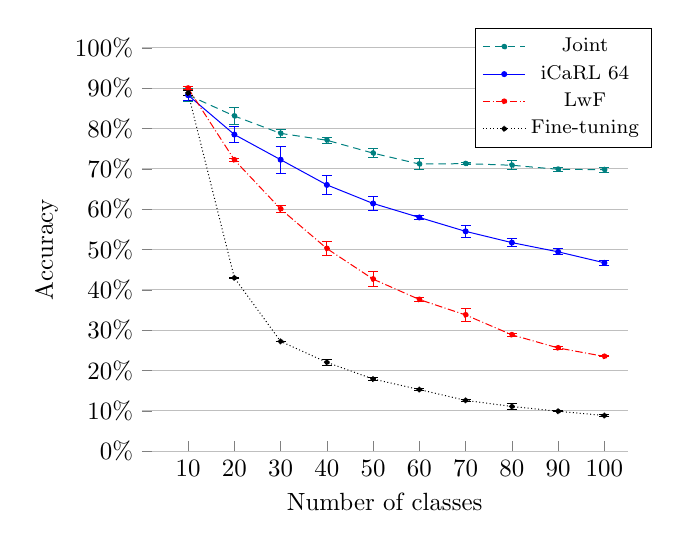
\begin{tikzpicture}[scale=0.90]
\begin{axis}[
        axis line style={draw=none},
        xmin=0, xmax=105,
        xtick={10,20,...,100},
        tick pos=left,
        ymin=0, ymax=1,
        ytick={0,0.1,0.2,0.3,0.4,0.5,0.6,0.7,0.8,0.9,1.0},
        yticklabel={\pgfmathparse{\tick*100}\pgfmathprintnumber{\pgfmathresult}\%},
        point meta={y*100},
        xlabel=Number of classes,
        ylabel=Accuracy,
        legend style={font=\footnotesize, at={(1.05,1.05)}, anchor=north east},
        ymajorgrids=true
    ]

    % Joint
    \addplot+[
        teal,
        mark=*,
        densely dashed,
        mark options={scale=0.5},
        error bars/.cd,
            y fixed,
            y dir=both,
            y explicit,
            error bar style={solid}
    ] table [x=x, y=y,y error=error, col sep=comma] {
        x,  y,       error
        10, 0.883, 0.016,
        20, 0.831, 0.021,
        30, 0.788, 0.009,
        40, 0.771, 0.007,
        50, 0.739, 0.012,
        60, 0.712, 0.013,
        70, 0.713, 0.002,
        80, 0.709, 0.011,
        90, 0.699, 0.005,
        100, 0.698, 0.006
    };

    % iCaRL scores
    \addplot+[
        blue,
        mark=*,
        mark options={scale=0.5},
        error bars/.cd,
            y fixed,
            y dir=both,
            y explicit,
            error bar style={solid}
    ] table [x=x, y=y,y error=error, col sep=comma] {
        x,  y,       error
        10, 0.88266667, 0.01228368,
        20, 0.78516667, 0.02002637,
        30, 0.72277778, 0.03299532,
        40, 0.66033333, 0.02372967,
        50, 0.61426667, 0.0181272,
        60, 0.57961111, 0.00563773,
        70, 0.54514286, 0.01427571,
        80, 0.51729167, 0.01019923,
        90, 0.49444444, 0.00730353,
        100, 0.46723333, 0.00642512
    };

    % LwF 2 scores
    \addplot+[
        red,
        densely dash dot,
        mark=*,
        mark options={scale=0.5},
        error bars/.cd,
            y fixed,
            y dir=both,
            y explicit,
            error bar style={solid}
    ] table [x=x, y=y,y error=error, col sep=comma] {
        x,  y,       error
        10, 0.90000, 0.00300,
        20, 0.72225, 0.00275,
        30, 0.60067, 0.00833,
        40, 0.50250, 0.01700,
        50, 0.42680, 0.01800,
        60, 0.37625, 0.00558,
        70, 0.33800, 0.01614,
        80, 0.28875, 0.00325,
        90, 0.25617, 0.00350,
        100, 0.23515, 0.00135
    };

    % Fine-tuning scores
    \addplot+[
        black,
        densely dotted,
        mark=*,
        mark options={scale=0.5},
        error bars/.cd,
            y fixed,
            y dir=both,
            y explicit,
            error bar style={solid}
    ] table [x=x, y=y,y error=error, col sep=comma] {
        x,  y,       error
        10, 8.88000000e-01, 6.00000000e-03,
        20, 4.30000000e-01, 1.50000000e-03,
        30, 2.72500000e-01, 8.33333333e-04,
        40, 2.20500000e-01, 7.25000000e-03,
        50, 1.79200000e-01, 3.20000000e-03,
        60, 1.53083333e-01, 2.25000000e-03,
        70, 1.26285714e-01, 1.57142857e-03,
        80, 1.11187500e-01, 7.68750000e-03,
        90, 9.93333333e-02, 1.44444444e-03,
        100, 8.87500000e-02, 3.25000000e-03
    };

    \addlegendentry{Joint}
    \addlegendentry{iCaRL $64$}
    \addlegendentry{LwF}
    \addlegendentry{Fine-tuning}
\end{axis}
\end{tikzpicture}
\caption{Accuracy comparison of the implemented baselines and upper bound. iCaRL outperforms both Learning without Forgetting and fine-tuning. The gap between the methods increases and the curves become flatter as more incremental steps are taken.}
\label{fig:experiments:plot}
\end{figure}

\subsection{Joint Training}
Our first experiment violates the incremental learning protocol. At each learning step, the network is trained not only on the current batch of classes, but on the union of all batches seen until that point. Therefore, we get an upper bound for the classification accuracy at each incremental step.

\subsection{Fine-tuning}
The first incremental learning baseline is a naive fine-tuning approach. This method is useful to understand how catastrophic forgetting affects the accuracy of a model in the incremental learning setting. We use the validation set to choose the network that minimizes the validation loss. This network is then used to evaluate the model on the current test set.

We use the binary cross entropy (BCE) loss function with one-hot encoded targets as the only contribution to the loss function. At each learning step, we optimize our network for the new classification task. The weights learned at the previous step are effectively the initialization for the new task network. As there is no mechanism to preserve previous knowledge, the optimization function updates the weights with the only goal of correctly classifying the current batch. In doing so, it makes the current weights less suitable for classifying old classes. This is how catastrophic forgetting occurs.

Figure~\ref{fig:experiments:plot} shows that fine-tuning is the least effective method among the baselines. The classification accuracy drops significantly at the end of the second learning step, and keeps decreasing as the number of classes grow. The accuracy of the model at the last batch hovers around 10\%, which suggests it is able to properly classify only the last batch of classes. The confusion matrix in Figure~\ref{fig:experiments:confmat} confirms this observation.

\subsection{Learning without Forgetting}
As a first step to mitigate the effects of catastrophic forgetting, we implement the Learning without Forgetting \cite{li:2016} framework. The novelty of this approach is the addition of the distillation loss, as presented in \cite{hinton:2015}. Knowledge distillation consists in transferring knowledge from the previous network to the current one. We copy and freeze the previous network and then train on the new batch of data. We use this training data to obtain outputs from the previous network and we use these outputs as targets for the training network. The network is encouraged to reproduce the probability scores of the old network by a distillation loss.

Differently from the Learning without Forgetting paper, we use the BCE loss for both the distillation and classification contributions. We are favouring the loss function of iCaRL to achieve better performance, as we demonstrate with our experiments on loss functions in Section~\ref{section:loss}.

Figure~\ref{fig:experiments:plot} shows a noteworthy increase in classification accuracy. By introducing a distillation loss contribution, Learning without Forgetting reaches an average incremental accuracy of $46.4\%$, while fine-tuning only scores $25.2\%$, highlighting the effectiveness of knowledge distillation. This is confirmed by the confusion matrix in Figure~\ref{fig:experiments:confmat}.

\subsection{iCaRL}
The final baseline for incremental learning consists in the iCaRL \cite{rebuffi:2017} algorithm. Besides using knowledge distillation, iCaRL introduces two novel components to address the shortcomings of the previous approaches. Firstly, it stores in memory K exemplars from old classes, augmenting the training dataset. It uses this additional training data to rehearse previously gained knowledge, limiting the effects of catastrophic forgetting. The size of the exemplars set K is fixed, so the memory footprint of the algorithm remains bounded. Secondly, it introduces a \emph{nearest-mean-of-exemplars} (NME) classifier. In this setting, the network is treated as a feature extractor up to the second to last layer. To classify an unlabeled sample, iCaRL computes a prototype vector for each class observed so far and the feature vector of the image to classify, and assigns the class label of the most similar prototype.

The NME classifier is a valuable addition that results in a significant increase in classification accuracy. To understand the impact of this component, we reproduced the differential analysis of the iCaRL paper by creating a hybrid setup that learns a representation in the same way as iCaRL, but uses the outputs of the last fully connected layer for classification instead of the NME classifier. This is referred to \emph{hybrid1} in the original paper and in our study as well. The results of our experiments show that NME increases the average incremental accuracy by $4.7\%$, as reported in Table~\ref{tab:experiments}.

The loss function used by iCaRL presents a distillation term that encourages the network to reproduce the scores of the old network for previous classes, and a classification term to output the correct class label for new classes.

In our implementation of iCaRL, we do not apply any data augmentation to the exemplars set in order to better preserve the original mean when computing the class prototype. We find that this marginally improves the classification performance of NME. Furthermore, we do not perform herding, \ie, prioritized exemplars selection, but randomly sample exemplars from the current batch of data without replacement. This approach is computationally less expensive than herding and improves the average incremental accuracy by $1.8\%$, compared to using the original iCaRL approach. We do not modify any other part of the exemplars handling algorithm.

\begin{table}
    \begin{center}
        \begin{tabular}{|r|c|}
        \hline
        Method & Avg. \\
        \hline\hline
        Fine-tuning & $25.7\%$ \\
        LwF & $46.4\%$ \\
        iCaRL &  $62.7\%$ \\
        hybrid1 &  $58.0\%$ \\
        \hline
        \end{tabular}
    \end{center}
\caption{Comparison between results with fine-tuning, Learning without Forgetting, our implementation of iCaRL and hybrid1 in terms of average incremental accuracy.
}
\label{tab:experiments}
\end{table}

Note that our results are $1.5\%$ lower than those reported by the authors of iCaRL. This difference may be due to the fact that the authors implement their algorithm using TensorFlow and Theano, while our code is based on PyTorch. This may also explain why we obtain better results by halving the original mini-batch size.

%%%%%%%%%%%%%%%%%%%%%%%%%%%%%
\section{Loss Ablation Study}
%%%%%%%%%%%%%%%%%%%%%%%%%%%%%
\label{section:loss}

In this section we mainly focus on loss functions. We want to observe the behaviour of the network as we replace the classification and distillation losses with different combinations. We mostly use the iCaRL framework as a baseline for our experiments, as it builds on the insights of Learning without Forgetting to increase the classification performance. In fact, it is the best performing method among all the evaluated incremental learning baselines.

This class of experiments is mainly devoted to understanding the behaviour and limitations of the existing frameworks, rather than trying to increase the accuracy of the baselines.

\subsection{Learning without Forgetting}
\label{section:loss:lwf}
\begin{figure}
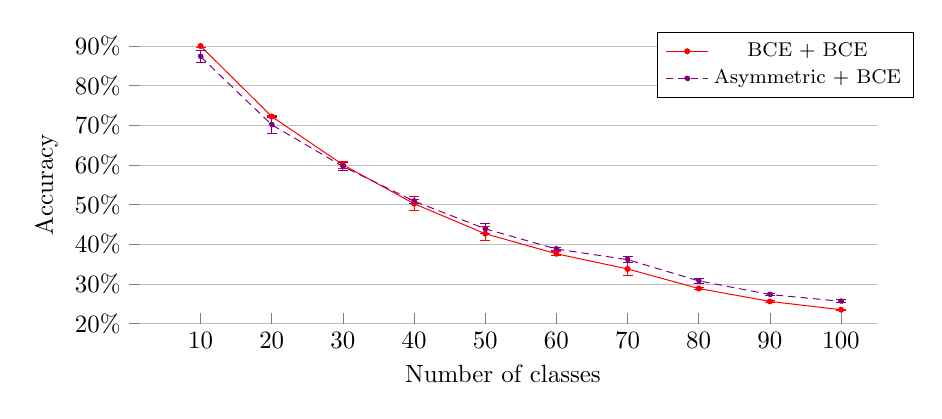
\begin{tikzpicture}[scale=0.9]
\begin{axis}[
        width=\columnwidth,
        height=5.5cm,
        axis line style={draw=none},
        xmin=0, xmax=105,
        xtick={10,20,...,100},
        tick pos=left,
        ymin=0.2, ymax=0.9,
        ytick={0.2,0.3,0.4,0.5,0.6,0.7,0.8,0.9},
        yticklabel={\pgfmathparse{\tick*100}\pgfmathprintnumber{\pgfmathresult}\%},
        point meta={y*100},
        xlabel=Number of classes,
        ylabel=Accuracy,
        legend style={font=\footnotesize, at={(1.05,1.05)}, anchor=north east},
        ymajorgrids=true
    ]

    % LwF 2 scores
    \addplot+[
        red,
        mark=*,
        mark options={scale=0.5},
        error bars/.cd,
            y fixed,
            y dir=both,
            y explicit,
            error bar style={solid}
    ] table [x=x, y=y,y error=error, col sep=comma] {
        x,  y,       error
        10, 0.90000, 0.00300,
        20, 0.72225, 0.00275,
        30, 0.60067, 0.00833,
        40, 0.50250, 0.01700,
        50, 0.42680, 0.01800,
        60, 0.37625, 0.00558,
        70, 0.33800, 0.01614,
        80, 0.28875, 0.00325,
        90, 0.25617, 0.00350,
        100, 0.23515, 0.00135
    };

    % custom loss
    \addplot+[
        violet,
        densely dashed,
        mark=*,
        mark options={scale=0.5},
        error bars/.cd,
            y fixed,
            y dir=both,
            y explicit,
            error bar style={solid}
    ] table [x=x, y=y,y error=error, col sep=comma] {
        x,  y,       error
        10, 0.87333, 0.01511,
        20, 0.70150, 0.02118,
        30, 0.59633, 0.01109,
        40, 0.50900, 0.00500,
        50, 0.43920, 0.01300,
        60, 0.38825, 0.00275,
        70, 0.36150, 0.00850,
        80, 0.30800, 0.00600,
        90, 0.27350, 0.00350,
        100, 0.25650, 0.00350
    };

    \addlegendentry{BCE + BCE}
    \addlegendentry{Asymmetric + BCE}
\end{axis}
\end{tikzpicture}
\caption{Different accuracy reached in the Learning without Forgetting framework using our custom asymmetric loss for classification against a network that uses the BCE loss. The distillation loss is BCE for both methods.}
\label{fig:loss:lwf}
\end{figure}

We perform only one experiment with the Learning without Forgetting framework. We define a custom loss that addresses a criticality in our setting. Whenever we train a model, after a finite number of epochs, the non-zero probability scores assigned to classes other than the target bring valuable information related to the similarity between the target class and other classes. The usage of the BCE loss function for classification implies that penalization does not only occur for misclassification errors, \ie, when predictions differ from targets, but also when probabilities differ from exactly $0$ on all remaining classes, implying also penalization of some informative scores.

To clarify our reasoning, let us consider a toy classification problem with three classes: cat, dog and car. The cat class is more similar to dog than car. During training, whenever the model encounters a sample of cat, valuable similarity information is encoded in the probability ratios between cat and the other classes, as we expect the model to give a higher probability score to dog than to car.

To verify this intuition, we design an asymmetric classification loss function with different penalization assigned to targets $0$ and $1$:
\begin{equation}
    \mathcal{L}_{asym}=\sum_{y=s}^{t} -y \log{g(x)} + (1-y)\;(g(x))^{2} \label{eq:loss:asym}
\end{equation}
where $s, \dots, t$ are the new classes and $g(x)$ is the output of the sigmoid layer. Targets are passed to the function with one-hot encoding.

While BCE penalizes all targets $0$ logarithmically, the cross entropy (CE) loss considers only the single output node of the target class. Our classification loss (\ref{eq:loss:asym}) stands between these two, with a quadratic penalization of $0$ targets. We think that this formulation has an advantage over CE in the Learning without Forgetting framework, as it addresses the imbalance in contributions that occurs when the number of old classes grows. The classification loss becomes less and less important than the distillation part as more incremental learning steps are taken, because the distillation contribution involves an increasing number of output nodes. When this disproportion is high, the classification loss is not able to adequately learn to classify new classes and the performance of the network on the new batch decreases.

In this setting, using a sigmoid layer instead of a softmax function to transform the outputs of the last fully connected layer to a probability distribution is fundamental. The softmax function normalizes the outputs in such a way to guarantee that the sum of all outputs is $1$. On the other hand, the sigmoid layer simply maps the scores to the $[0, 1]$ range, assigning a probabilistic meaning to each output node activation independently from other ones. We present the results in Figure~\ref{fig:loss:lwf}.

\subsection{iCaRL}
\begin{figure}
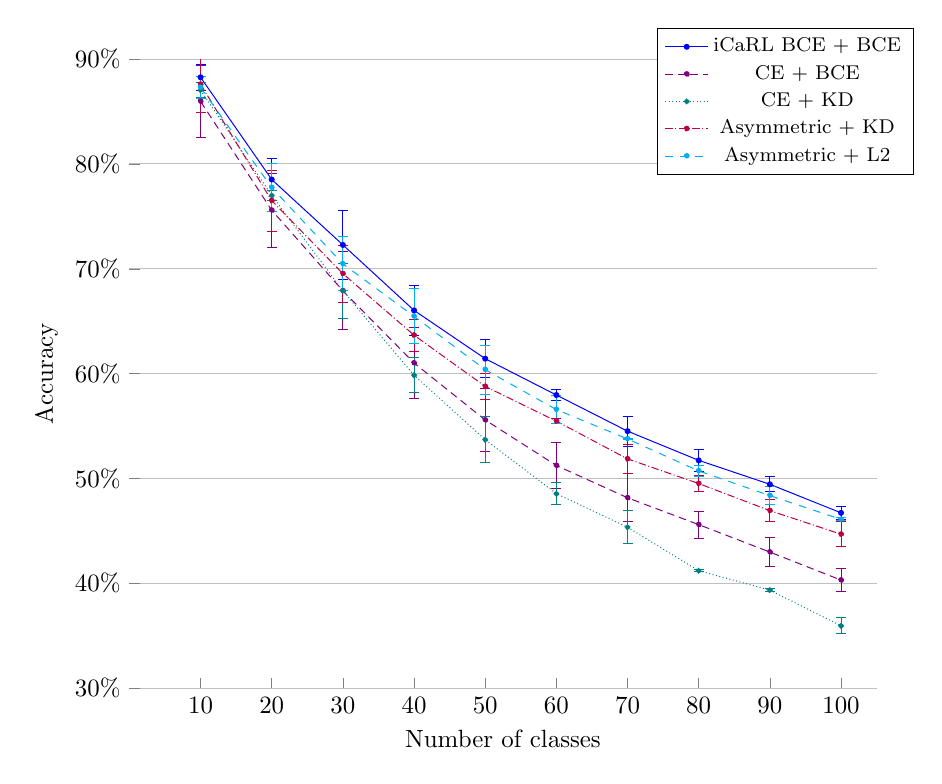
\begin{tikzpicture}[scale=0.9]
\begin{axis}[
        width=\columnwidth,
        axis line style={draw=none},
        xmin=0, xmax=105,
        xtick={10,20,...,100},
        tick pos=left,
        ymin=0.3, ymax=0.9,
        ytick={0.3,0.4,0.5,0.6,0.7,0.8,0.9},
        yticklabel={\pgfmathparse{\tick*100}\pgfmathprintnumber{\pgfmathresult}\%},
        point meta={y*100},
        xlabel=Number of classes,
        ylabel=Accuracy,
        legend style={font=\footnotesize, at={(1.05,1.05)}, anchor=north east},
        ymajorgrids=true
    ]

    % iCaRL scores (baseline)
    \addplot+[
        blue,
        mark=*,
        mark options={scale=0.5},
        error bars/.cd,
            y fixed,
            y dir=both,
            y explicit,
            error bar style={solid}
    ] table [x=x, y=y,y error=error, col sep=comma] {
        x,  y,       error
        10, 0.88266667, 0.01228368,
        20, 0.78516667, 0.02002637,
        30, 0.72277778, 0.03299532,
        40, 0.66033333, 0.02372967,
        50, 0.61426667, 0.0181272,
        60, 0.57961111, 0.00563773,
        70, 0.54514286, 0.01427571,
        80, 0.51729167, 0.01019923,
        90, 0.49444444, 0.00730353,
        100, 0.46723333, 0.00642512
    };

    % CE + BCE
    \addplot+[
        violet,
        densely dashed,
        mark=*,
        mark options={scale=0.5},
        error bars/.cd,
            y fixed,
            y dir=both,
            y explicit,
            error bar style={solid}
    ] table [x=x, y=y,y error=error, col sep=comma] {
        x,  y,       error
        10, 0.85967, 0.03462,
        20, 0.75583, 0.03510,
        30, 0.67900, 0.03735,
        40, 0.61017, 0.03365,
        50, 0.55580, 0.03012,
        60, 0.51239, 0.02203,
        70, 0.48157, 0.02272,
        80, 0.45600, 0.01279,
        90, 0.42981, 0.01387,
        100, 0.40310, 0.01134
    };

    % CE + KD
    \addplot+[
        teal,
        densely dotted,
        mark=*,
        mark options={scale=0.5},
        error bars/.cd,
            y fixed,
            y dir=both,
            y explicit,
            error bar style={solid}
    ] table [x=x, y=y,y error=error, col sep=comma] {
        x,  y,       error
        10, 0.87050, 0.00750,
        20, 0.77000, 0.00500,
        30, 0.67900, 0.02600,
        40, 0.59850, 0.01650,
        50, 0.53700, 0.02200,
        60, 0.48550, 0.01050,
        70, 0.45350, 0.01550,
        80, 0.41200, 0.00100,
        90, 0.39350, 0.00150,
        100, 0.35950, 0.00750
    };

    % Asymmetric + KD
    \addplot+[
        purple,
        densely dash dot,
        mark=*,
        mark options={scale=0.5},
        error bars/.cd,
            y fixed,
            y dir=both,
            y explicit,
            error bar style={solid}
    ] table [x=x, y=y,y error=error, col sep=comma] {
        x,  y,       error
        10, 0.87600, 0.02677,
        20, 0.76500, 0.02909,
        30, 0.69533, 0.02735,
        40, 0.63667, 0.01528,
        50, 0.58780, 0.01242,
        60, 0.55467, 0.00249,
        70, 0.51867, 0.01372,
        80, 0.49517, 0.00792,
        90, 0.46933, 0.01066,
        100, 0.44683, 0.01206
    };

    % Asymmetric + L2
    \addplot+[
        cyan,
        dashed,
        mark=*,
        mark options={scale=0.5},
        error bars/.cd,
            y fixed,
            y dir=both,
            y explicit,
            error bar style={solid}
    ] table [x=x, y=y,y error=error, col sep=comma] {
        x,  y,       error
        10, 0.87300, 0.01020,
        20, 0.77750, 0.02327,
        30, 0.70467, 0.02582,
        40, 0.65467, 0.02634,
        50, 0.60380, 0.02348,
        60, 0.56567, 0.01352,
        70, 0.53771, 0.00051,
        80, 0.50721, 0.00524,
        90, 0.48367, 0.00834,
        100, 0.46100, 0.00141
    };

    \addlegendentry{iCaRL BCE + BCE}
    \addlegendentry{CE + BCE}
    \addlegendentry{CE + KD}
    \addlegendentry{Asymmetric + KD}
    \addlegendentry{Asymmetric + L2}
\end{axis}
\end{tikzpicture}
\caption{Representation of test accuracy of the iCaRL framework with different loss function pairings. The choice of the loss function is not negligible, resulting in about $10\%$ difference of average incremental accuracy on the last split between BCE + BCE and CE + KD. We also see how the CE loss for classification is always giving the worst performance.}
\label{fig:loss:plot}
\end{figure}

\subsubsection{CE + BCE}
\label{section:loss:cebce}
The first combination of classification and distillation loss functions that we implement in the iCaRL framework is CE and BCE. In Section~\ref{section:loss:lwf} we explain how these two contributions are unbalanced. In particular, we show how the CE contribute loses of importance as more learning steps are taken, due to the increasing number of output nodes for old classes. The inability to adequately learn new classes exhibits as an accuracy drop with respect to the baseline, as we show in Figure~\ref{fig:loss:plot}.

\subsubsection{CE + Knowledge Distillation}
The second experiment that we perform involves the knowledge distillation loss introduced by \cite{hinton:2015}. The combination of this distillation loss with CE for classification is in line with the original implementation of the LWF framework. We want to understand whether the use of BCE for both classification and distillation is sensible by performing this experiment, also given the conclusions drawn in Section~\ref{section:loss:cebce}.

The knowledge distillation loss presented by \cite{hinton:2015} can be interpreted as a modified CE loss:
\begin{equation}
    \mathcal{L}_{old}(y_{o}, \hat{y}_{o})=-H(y_{o}', \hat{y}_{o}')=-\sum_{i=1}^{l} y_{o}'^{(i)} \log{\hat{y}_{o}'^{(i)}} \label{eq:loss:cebce}
\end{equation}
where $l$ is the number of old classes and $y_{o}'^{(i)}, \hat{y}_{o}'^{(i)}$ are the modified versions of old and current probabilities $y_{o}^{(i)}, \hat{y}_{o}^{(i)}$:
\begin{equation}
    y_{o}'^{(i)}=\frac{(y_{o}^{(i)})^{1/T}}{\sum_{j} (y_{o}^{(j)})^{1/T}}, \qquad \hat{y}_{o}'^{(i)}=\frac{(\hat{y}_{o}^{(i)})^{1/T}}{\sum_{j} (\hat{y}_{o}^{(j)})^{1/T}}. \label{eq:loss:cebce2}
\end{equation}

$T$ is an hyper-parameter called temperature, which is set to $1$ in the standard softmax function. We use $T > 1$ to produce \emph{soft targets}, \ie, a probability distribution more equally spread among the old classes. This is in accordance with \cite{hinton:2015}, as to distill knowledge a set of soft targets with high entropy provide much more information than hard targets.

We set $T = 2$ as in the official Learning without Forgetting implementation. In Figure~\ref{fig:loss:plot} we compare results given by our combination of losses and BCE for both classification and distillation. Table~\ref{tab:loss} shows a $7\%$ drop of average incremental accuracy. This difference may be explained by our reasoning on the limits of CE as a classification loss for the incremental learning task. Moreover, using a sigmoid function naturally produces softer targets, since the sum of probabilities between all classes is not constrained to $1$ as it is for softmax.

\begin{table}
    \begin{center}
        \begin{tabular}{|r|c|}
        \hline
        Method & Avg. \\
        \hline\hline
        Asymmetric + BCE (LwF) & $47.1\%$ \\
        CE + BCE & $57.4\%$ \\
        CE + KD &  $55.6\%$ \\
        Asymmetric + BCE &  $60.5\%$ \\
        Asymmetric + L2 &  $61.7\%$ \\
        \hline
        \end{tabular}
    \end{center}
\caption{Comparison of the average incremental accuracy of different combinations of loss functions. The first combination refers to the Learning without Forgetting algorithm, while all the other ones are implemented using iCaRL.}
\label{tab:loss}
\end{table}

\subsubsection{Asymmetric + BCE}
\label{asymbce}
Our next study consists in substituting the classification loss of iCaRL with our custom asymmetric loss (\ref{eq:loss:asym}), while keeping BCE as our distillation loss. We aim at mitigating the limitations of the CE loss (see Section~\ref{section:loss:lwf}) for the incremental learning task and evaluating the behaviour of the network with this intermediate approach. We also investigate whether this classification loss is able to outperform the baseline iCaRL implementation, as it did with the Learning without Forgetting algorithm.

In Figure~\ref{fig:loss:plot} we show that the current combination of loss functions results in weaker performance than the baseline, losing $2.2\%$ average incremental accuracy. We point out two main reasons to explain this result. The first reason is the imbalance between the classification and distillation loss contributions, that causes difficulties in learning new classes as more learning steps are taken. This imbalance is due to the fact that (\ref{eq:loss:asym}) presents a quadratic term, while BCE has a logarithmic term. The second reason is that the intuition behind the design of our custom asymmetric loss may not be valid anymore. With an increasing number of known classes, the probabilities associated to wrong labels may lose the similarity meaning that we pointed out. Therefore, they need a harsher penalization.

\subsubsection{Asymmetric + L2}
The last experiment with loss functions consists in our custom asymmetric loss function (\ref{eq:loss:asym}) as the classification loss, and L2 as the distillation loss. One of the issues identified in Section~\ref{asymbce} is the penalization imbalance between BCE and (\ref{eq:loss:asym}), in favour of the former. By modifying the distillation loss, we hope to strike a good balance between the two loss components.

In Figure~\ref{fig:loss:plot} we compare the results given by the current pair of loss functions and the combination of two BCE losses. We lose only $0.9\%$ average incremental accuracy on the evaluation set. In fact, the plot shows that the results given by these two loss combinations are very similar.

At the end of these ablation studies, having evaluated different classification and distillation loss combinations, we acknowledge that a pair of BCE losses appears to be the most suitable choice for the iCaRL algorithm.

%%%%%%%%%%%%%%%%%%%%%%%%%%%%%
\section{Classifier Ablation Study}
%%%%%%%%%%%%%%%%%%%%%%%%%%%%%
\label{section:classifier}

\begin{figure*}
\begin{center}
    \captionsetup[subfigure]{justification=centering}
    \begin{subfigure}{.24\textwidth}
        \centering
        \begin{tikzpicture}[scale=0.6]
        \begin{axis}[
            enlargelimits=false,
            axis on top,
            axis equal image,
            axis line style={draw=none},
            xmin=0, xmax=100,
            ymin=0, ymax=100,
            xtick={10,20,...,100},
            ytick={10,20,...,100},
            tick label style={major tick length=0pt},
            y dir=reverse,
            xlabel=Predicted class,
            % style={font=\footnotesize}
        ]
        \addplot graphics [
            xmin=0, xmax=100,
            ymin=0, ymax=100,
        ] {img/classifier/knn_all};
        \end{axis}
        \end{tikzpicture}
        \caption{k-NN all data}
        \label{fig:experiments:confmat:knn_all}
        \vspace*{5mm}
    \end{subfigure}
    \begin{subfigure}{.24\textwidth}
        \centering
        \begin{tikzpicture}[scale=0.6]
        \begin{axis}[
            enlargelimits=false,
            axis on top,
            axis equal image,
            axis line style={draw=none},
            xmin=0, xmax=100,
            ymin=0, ymax=100,
            xtick={10,20,...,100},
            ytick={10,20,...,100},
            tick label style={major tick length=0pt},
            y dir=reverse,
            xlabel=Predicted class,
            % style={font=\footnotesize}
        ]
        \addplot graphics [
            xmin=0, xmax=100,
            ymin=0, ymax=100,
        ] {img/classifier/knn_exemplars};
        \end{axis}
        \end{tikzpicture}
        \caption{k-NN exemplars}
        \label{fig:experiments:confmat:knn_exemplars}
        \vspace*{5mm}
    \end{subfigure}
    \begin{subfigure}{.24\textwidth}
        \centering
        \begin{tikzpicture}[scale=0.6]
        \begin{axis}[
            enlargelimits=false,
            axis on top,
            axis equal image,
            axis line style={draw=none},
            xmin=0, xmax=100,
            ymin=0, ymax=100,
            xtick={10,20,...,100},
            ytick={10,20,...,100},
            tick label style={major tick length=0pt},
            y dir=reverse,
            xlabel=Predicted class,
            % style={font=\footnotesize}
        ]
        \addplot graphics [
            xmin=0, xmax=100,
            ymin=0, ymax=100,
        ] {img/classifier/cosine_fc};
        \end{axis}
        \end{tikzpicture}
        \caption{Cosine layer}
        \label{fig:experiments:confmat:cosine_fc}
        \vspace*{5mm}
    \end{subfigure}

    \begin{subfigure}{.24\textwidth}
        \centering
        \begin{tikzpicture}[scale=0.6]
        \begin{axis}[
            enlargelimits=false,
            axis on top,
            axis equal image,
            axis line style={draw=none},
            xmin=0, xmax=100,
            ymin=0, ymax=100,
            xtick={10,20,...,100},
            ytick={10,20,...,100},
            tick label style={major tick length=0pt},
            y dir=reverse,
            xlabel=Predicted class,
            % style={font=\footnotesize}
        ]
        \addplot graphics [
            xmin=0, xmax=100,
            ymin=0, ymax=100,
        ] {img/classifier/cosine_sim};
        \end{axis}
        \end{tikzpicture}
        \caption{Cosine similarity}
        \label{fig:experiments:confmat:cosine_sim}
    \end{subfigure}
    \begin{subfigure}{.24\textwidth}
        \centering
        \begin{tikzpicture}[scale=0.6]
        \begin{axis}[
            enlargelimits=false,
            axis on top,
            axis equal image,
            axis line style={draw=none},
            xmin=0, xmax=100,
            ymin=0, ymax=100,
            xtick={10,20,...,100},
            ytick={10,20,...,100},
            tick label style={major tick length=0pt},
            y dir=reverse,
            xlabel=Predicted class,
            % style={font=\footnotesize}
        ]
        \addplot graphics [
            xmin=0, xmax=100,
            ymin=0, ymax=100,
        ] {img/classifier/rf_all};
        \end{axis}
        \end{tikzpicture}
        \caption{RF all data}
        \label{fig:experiments:confmat:rf_all}
    \end{subfigure}
    \begin{subfigure}{.24\textwidth}
        \centering
        \begin{tikzpicture}[scale=0.6]
        \begin{axis}[
            enlargelimits=false,
            axis on top,
            axis equal image,
            axis line style={draw=none},
            xmin=0, xmax=100,
            ymin=0, ymax=100,
            xtick={10,20,...,100},
            ytick={10,20,...,100},
            tick label style={major tick length=0pt},
            y dir=reverse,
            xlabel=Predicted class,
            % style={font=\footnotesize}
        ]
        \addplot graphics [
            xmin=0, xmax=100,
            ymin=0, ymax=100,
        ] {img/classifier/rf_exemplars};
        \end{axis}
        \end{tikzpicture}
        \caption{RF exemplars}
        \label{fig:experiments:confmat:rf_exemplars}
    \end{subfigure}
\caption{Confusion matrices of different classifiers on the incremental version of CIFAR-100. Training k-NN on the union of the exemplars dataset and the current training data results in more misclassification errors due to the higher number of data points belonging to the last ten classes. The cosine layer produces a confusion matrix similar to hybrid1, while the modified NME with cosine similarity retains a very good classification performance on old classes. Similarly to k-NN, the random forest classifier performs well when trained on a balanced dataset, while heavily skewing predictions towards the last ten classes when trained on all available training data.}
\label{fig:classifier:confmat}
\end{center}
\end{figure*}

We shift our focus to classifiers and evaluate several classification strategies. Our experiments aim at evaluating the performance of different classifiers and possibly finding a better alternative to the NME proposed by the authors of iCaRL. Therefore, we use NME as a baseline against which we compare all classifiers. The strategy we employ is to treat the network up to the second to last layer as a feature extractor $\varphi: \chi \to \mathbb{R}^{d}$, and use these features as inputs for the classifier. This is also how the authors of iCaRL implemented the NME classifier.

\begin{figure}
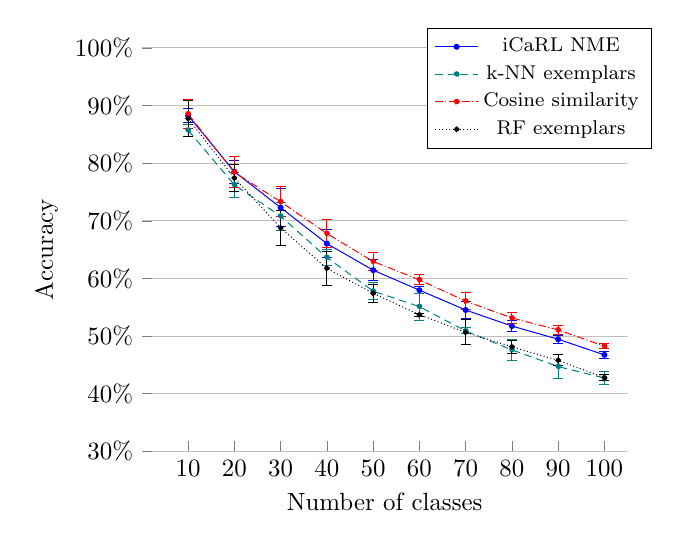
\begin{tikzpicture}[scale=0.90]
\begin{axis}[
        axis line style={draw=none},
        xmin=0, xmax=105,
        xtick={10,20,...,100},
        tick pos=left,
        ymin=0.3, ymax=1,
        ytick={0.3,0.4,0.5,0.6,0.7,0.8,0.9,1.0},
        yticklabel={\pgfmathparse{\tick*100}\pgfmathprintnumber{\pgfmathresult}\%},
        point meta={y*100},
        xlabel=Number of classes,
        ylabel=Accuracy,
        legend style={font=\footnotesize, at={(1.05,1.05)}, anchor=north east},
        ymajorgrids=true
    ]

    % iCaRL scores (baseline)
    \addplot+[
        blue,
        mark=*,
        mark options={scale=0.5},
        error bars/.cd,
            y fixed,
            y dir=both,
            y explicit,
            error bar style={solid}
    ] table [x=x, y=y,y error=error, col sep=comma] {
        x,  y,       error
        10, 0.88266667, 0.01228368,
        20, 0.78516667, 0.02002637,
        30, 0.72277778, 0.03299532,
        40, 0.66033333, 0.02372967,
        50, 0.61426667, 0.0181272,
        60, 0.57961111, 0.00563773,
        70, 0.54514286, 0.01427571,
        80, 0.51729167, 0.01019923,
        90, 0.49444444, 0.00730353,
        100, 0.46723333, 0.00642512
    };

    % k-NN
    \addplot+[
        teal,
        mark=*,
        densely dashed,
        mark options={scale=0.5},
        error bars/.cd,
            y fixed,
            y dir=both,
            y explicit,
            error bar style={solid}
    ] table [x=x, y=y,y error=error, col sep=comma] {
        x,  y,       error
        10, 0.857     , 0.01067708,
        20, 0.76233333, 0.0215109,
        30, 0.70788889, 0.024480,
        40, 0.63641667, 0.01437929,
        50, 0.57793333, 0.01515461,
        60, 0.55105556, 0.02353498,
        70, 0.50885714, 0.0051547,
        80, 0.47591667, 0.01872007,
        90, 0.447     , 0.02147426,
        100, 0.42713333 ,0.01048883
    };

    % Cosine
    \addplot+[
        red,
        densely dash dot,
        mark=*,
        mark options={scale=0.5},
        error bars/.cd,
            y fixed,
            y dir=both,
            y explicit,
            error bar style={solid}
    ] table [x=x, y=y,y error=error, col sep=comma] {
        x,  y,       error
        10, 0.88533, 0.02542,
        20, 0.78400, 0.02678,
        30, 0.73300, 0.02604,
        40, 0.67783, 0.02396,
        50, 0.62940, 0.01593,
        60, 0.59750, 0.00878,
        70, 0.56057, 0.01492,
        80, 0.53133, 0.00878,
        90, 0.51059, 0.00794,
        100, 0.48237, 0.00404
    };

    % RF
    \addplot+[
        black,
        densely dotted,
        mark=*,
        mark options={scale=0.5},
        error bars/.cd,
            y fixed,
            y dir=both,
            y explicit,
            error bar style={solid}
    ] table [x=x, y=y,y error=error, col sep=comma] {
        x,  y,       error
        10, 0.87733, 0.03064,
        20, 0.77433, 0.02358,
        30, 0.68767, 0.03031,
        40, 0.61742, 0.02978,
        50, 0.57413, 0.01572,
        60, 0.53706, 0.00235,
        70, 0.50638, 0.02190,
        80, 0.48138, 0.01094,
        90, 0.45785, 0.00940,
        100, 0.42780, 0.00576
    };

    \addlegendentry{iCaRL NME}
    \addlegendentry{k-NN exemplars}
    \addlegendentry{Cosine similarity}
    \addlegendentry{RF exemplars}
\end{axis}
\end{tikzpicture}
\caption{Comparison of the iCaRL NME baseline against other classifiers. The only alternative classifier that outperforms iCaRL is the cosine layer with a modified NME with cosine similarity. Both k-NN and random forest perform worse.}
\label{fig:classifier:plot}
\end{figure}

\subsection{K-Nearest Neighbors}
The first classifier we evaluate is the k-nearest neighbors (k-NN) algorithm. It is an instance-based learning method that computes the class of unlabeled samples by the majority label among its k nearest neighbors in the training set.

Both the k-NN algorithm and NME adopt a distance-based approach to classification. NME computes the mean of each class observed so far and then measures the distance between the new image and the class means, assigning the label of the nearest class mean. In contrast, k-NN measures the distance between the new sample and all available labeled samples without computing any mean. To ensure a fair comparison, we use the L2 distance for k-NN.

The k-NN algorithm requires a normalized and balanced dataset to perform at its best. We scale the feature set to the range $[0, 1]$ in order for each feature to be of equal importance when computing the L2 distance. Moreover, we discard the additional samples available during training and fit the classifier on the exemplars dataset only. In this case, using a smaller but well balanced dataset is better than using a dataset with more samples with a distribution heavily skewed towards new classes, as we demonstrate in the results section. This problem does not arise in NME, as it computes only one prototype per class regardless of the number of samples per class.

\paragraph{Implementation.} After each incremental step, we extract features from the exemplar set and we fit the k-NN model on this data. We carry out a grid search to choose the best K and weight function at each incremental step, using the validation set to measure the accuracy of the models. We evaluate models with K equal to $3$, $5$, $7$ and $9$ and weight functions \emph{uniform} and \emph{distance}. The uniform function weights all points in each neighborhood equally, while the distance function weights points by the inverse of their distance, therefore points closer to the sample have a greater influence on classification.

We use the k-NN implementation provided by the \emph{scikit-learn} library.

\paragraph{Results.} We find that using k-NN for classification results in slightly worse accuracy than NME. Nevertheless, k-NN mitigates the effects of catastrophic forgetting reasonably well. We compare k-NN to other classifiers in Figure~\ref{fig:classifier:plot}. The difference in accuracy between k-NN and NME may be due to the fact that computing a class mean prototype reduces the detrimental effects of noise in the data.

As we can see by comparing the confusion matrices of k-NN in Figure~\ref{fig:classifier:confmat}, training the classifier on the union of exemplars and training data results in more test samples to be misclassified as belonging to one of the last ten classes. In fact, the probability that the K nearest neighbors of any sample belong to the majority classes becomes higher due to their higher density in the space, resulting in worse classification performance. Using an unbalanced dataset results in an average incremental accuracy of $54.1\%$, which is $5.3\%$ less than the accuracy of the model trained exclusively on the exemplars set.

\subsection{Cosine Similarity}
The second classifier we evaluate is a cosine normalization layer as described in \cite{hou:2019} paired with a modified NME that uses cosine similarity to compute distances. The study carried out in \cite{hou:2019} reveals that the imbalance between previous classes and new data is a crucial cause to catastrophic forgetting, and goes on to propose some solutions. We mainly focus on the cosine normalization layer and do not explore the effect of other proposed components, as they are outside the scope of the classifier ablation studies.

\begin{figure}
\begin{center}
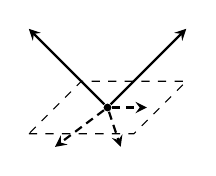
\begin{tikzpicture}
    \draw (3/3,-4/3) node[circle,fill,inner sep=1] (orig) {};

    \draw[->, >=stealth, thick] (orig) -- (0,-1/3);
    \draw[->, >=stealth, thick] (orig) -- (6/3,-1/3);

    \draw[dashed] (0,-5/3) -- (4/3,-5/3) -- (6/3,-3/3) -- (2/3,-3/3) -- (0,-5/3);

    \draw[->, >=stealth, thick, densely dashed] (orig) -- (1/3,-5.5/3);
    \draw[->, >=stealth, thick, densely dashed] (orig) -- (3.5/3,-5.5/3);
    \draw[->, >=stealth, thick, densely dashed] (orig) -- (4.5/3,-4/3);
\end{tikzpicture}
\qquad \qquad
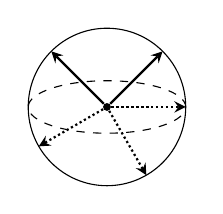
\begin{tikzpicture}
    % Define radius
    \def\r{1}

    % Bloch vector
    \draw (0,0) node[circle,fill,inner sep=1] (orig) {};

    % Sphere
    \draw (orig) circle (\r);
    \draw[dashed] (orig) ellipse (\r{} and \r/3);

    % Axes
    \draw[->, >=stealth, thick] (orig) -- ++(\r/1.41421,\r/1.41421) node {};
    \draw[->, >=stealth, thick] (orig) -- ++(-\r/1.41421,\r/1.41421) node {};

    \draw[->, >=stealth, thick, densely dotted] (orig) -- ++(\r,0) node {};
    \draw[->, >=stealth, thick, densely dotted] (orig) -- ++(-\r*0.866,-\r*0.5) node {};
    \draw[->, >=stealth, thick, densely dotted] (orig) -- ++(\r*0.5,-\r*0.866) node {};
\end{tikzpicture}
\end{center}
\caption{Illustration of the magnitude imbalance between previous classes and new data, which is a crucial cause to catastrophic forgetting, and how the cosine linear layer tackles this problem. Dashed lines represent old class embeddings and solid lines represent new ones.}
\label{fig:classifier:cosine:features}
\end{figure}

The authors observe that the magnitudes of the weight vectors and biases of new classes are higher than those of old classes. We are able to reproduce this harmful behaviour in iCaRL. The cosine layer solves this problem by enforcing balanced magnitudes across all classes, as illustrated in Figure~\ref{fig:classifier:cosine:features}. It replaces the last fully connected linear layer of the network, which computes the activations of its output neurons as described in (\ref{eq:1}), whereas the cosine layer measures the cosine similarity between two normalized vectors, computing the activations as (\ref{eq:2}):
\begin{align}
    \theta_{i}^{T} \varphi(x) + b_{i} \label{eq:1}\\
    \eta \langle \bar{\theta}_{i}^{T}, \bar{\varphi}(x) \rangle \label{eq:2}
\end{align}
where $v = v/\lVert v \rVert_{2}$ denotes the L2 normalized vector and $\langle v_{1}, v_{2} \rangle = v_{1}^{T} v_{2}$ measures the cosine similarity between two normalized vectors.

A natural choice for the classification strategy is to use the output of the network as is. However, we may improve this method by adopting an approach similar to iCaRL. We use a modified version of the NME that takes into account the different nature of the features by using the maximum cosine similarity instead of the minimum L-2 distance between the sample and the class prototypes. In other words, we change the computation of the nearest prototype in Algorithm 1 of iCaRL to (\ref{eq:3}).

\begin{equation}
    y^{*} \gets \argmax_{y=1, \dots, t} \langle \bar{\varphi}(x), \bar{\mu}_{y} \rangle \label{eq:3}
\end{equation}

where $y^{*}$ is the predicted label, $t$ is the total number of classes observed so far and $\mu_{y}$ is the prototype vector of the $y$-th class.

\paragraph{Implementation.} Firstly, we classify samples using the outputs of the cosine linear layer as they are. Then, we attempt to improve this method. Similarly to iCaRL, we extract features from the set of exemplars and compute a prototype per class. Then, we classify samples by a modified NME rule, calculating the cosine similarity between new images and prototypes.

\paragraph{Results.} We find that using the outputs of the cosine normalization layer produces results comparable to hybrid1, only marginally higher towards the last incremental steps, reaching an average incremental accuracy of $58.4\%$. Figure~\ref{fig:classifier:confmat} illustrates the similarities of the confusion matrices as well, showing that new classes are frequently misclassified as old classes. The relatively low accuracy of the cosine layer compared to other classifiers may be due to not having implemented the additional components proposed in \cite{hou:2019}, which are instrumental to obtain higher performance.

Nevertheless, we find that NME with cosine similarity outperforms iCaRL, as shown in Figure~\ref{fig:classifier:plot}. This confirms that unbalanced magnitudes of the weight vectors between old and new classes play a role in catastrophic forgetting, and that the cosine layer effectively eliminates the bias caused by the difference in magnitudes, increasing the classification accuracy. The average incremental accuracy of the cosine similarity model is $63.9\%$, which is $1.2\%$ above iCaRL.

\subsection{Random Forest}
The last classifier we test is a random forest \cite{breiman:2001}, an ensemble learning method based on decision trees. A random forest exploits the insight that an ensemble with many relatively uncorrelated models has better predictive capability than any of its components. This set of models is built by introducing randomness in their construction through bootstrap aggregation (\emph{bagging}) and feature selection, effectively reducing the variance of the estimator. The prediction is given by an average across all classifiers. We are interested in seeing how this model differs from the other distance-based classification approaches.

The decision trees in the ensemble are built by repeatedly sampling with replacement the training data, \ie, extracting bootstrap samples from the current batch of classes. Moreover, each decision tree is built using a random subset of $\sqrt{d}$ features, with $d$ the total number of features. This number empirically gives good results for classification tasks. The resulting decision trees are relatively uncorrelated, reducing the overall variance of the ensemble. As we only use a subset of training data for each decision tree, bias is likely to increase. However, the concurrent decrease in variance usually results in better classification accuracy, good generalization ability and robustness with respect to noise.

Decision trees are very sensitive to imbalanced training data, so we expect a random forest to perform poorly if trained on the union of the exemplars set and the current training data. Therefore, we also build a random forest trained only on the exemplars set.

\paragraph{Implementation.}
After each incremental step, we fit the ensemble on features extracted from the exemplars set. We carry out a grid search to choose the best number of estimators among $100$, $200$, $500$ and $1000$, and the minimum number of samples required to split an internal node among $10$, $20$ and $50$. The latter parameter is useful to limit overfitting in the decision trees.

We use the random forest classifier implementation provided by the \emph{scikit-learn} library.

\paragraph{Results.}
We find that the random forest trained exclusively on the exemplars set results in worse accuracy than NME. The average incremental accuracy is $59.4\%$, which is the lowest score among all classifiers. 

As we expected, training a random forest on the union of exemplars and training data results in a higher misclassification error, with predictions skewed towards the last ten classes as we can see in Figure~\ref{fig:classifier:confmat}. The average incremental accuracy of this model suffers from a significant drop to $44.3\%$, which is $15.1\%$ less than the one trained only on the exemplars set.

%%%%%%%%%%%%%%%%%%%%%%%%%%%%%%
\section{Beyond the Baselines}
%%%%%%%%%%%%%%%%%%%%%%%%%%%%%%

We dedicate this last section to studying more deeply some of the existing limitations in the incremental learning frameworks, and we propose some measures to attempt to mitigate them.

\subsection{Distillation Targets Study}
Every time the network receives a new batch of classes, we take a further incremental training step. In our setting, we need ten steps for our final model to learn all the classes contained in the original dataset. Targets for the distillation loss at step $N$ are obtained from the network trained at step $N-1$, \ie, on the previous batch.

Consider a prediction node in the last fully connected layer, related to a class associated to batch $M<N-1$, where $M$ refers to any step older than the previous one. We hypothesize a significant difference between probabilities assigned by the network $N-1$ and the ones given by the network $M$. In order to prove this, we save the trained network at each incremental step, which is used in the next task to produce distillation targets only for the classes it was specifically trained on, \ie, excluding the exemplars set. The loss function compares these scores with the one produced by the network at step $N-1$.

In Figure~\ref{100a}, we show the difference between distillation targets produced by the baseline framework versus the ones given by our new policy, which we refer to as \emph{multi networks}. The scores are related to the ninth split, and all predictions are taken from a sample with label $0$. We may expect that both policies can effectively recognize the correct label of the sample. However, we can observe a more spread distribution with respect to the one given by the last network. Since each model is an expert in recognizing data it was trained on, its predictions are more confident and therefore closer to $0$. In some cases, the target gap between the policies can reach $6$ order of magnitudes.

\begin{figure}
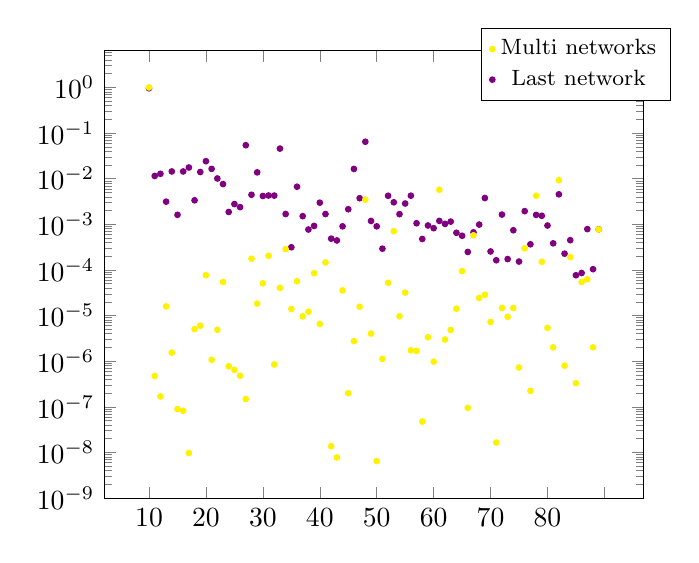
\begin{tikzpicture}
\begin{axis}[
    scatter/classes={
        old={mark=*,mark size=1pt,yellow},
        last={mark=*,mark size=1pt,violet}},
        xticklabels={0,10,...,80},
        max space between ticks=20,
        legend style={font=\footnotesize, at={(1.05,1.05)}, anchor=north east},
        ymode=log
]
\addplot[scatter,only marks,%
    scatter src=explicit symbolic]%
        table[meta=label] {
        x y label
        0 0.9588 last
        1 0.0114788624 last
        2 0.012801765 last
        3 0.003142994 last
        4 0.01441521 last
        5 0.0016169614 last
        6 0.01443137 last
        7 0.0176103535 last
        8 0.0033608385 last
        9 0.014026096 last
        10 0.02422393 last
        11 0.016426644 last
        12 0.0101222067 last
        13 0.007634055 last
        14 0.00186699215 last
        15 0.00278246115 last
        16 0.0023820986 last
        17 0.054223065 last
        18 0.004444426 last
        19 0.013769971 last
        20 0.0041849474 last
        21 0.00428614485 last
        22 0.004263856 last
        23 0.0457139095 last
        24 0.00168346805 last
        25 0.000314604945 last
        26 0.0066756575 last
        27 0.00151063205 last
        28 0.00076936535 last
        29 0.000922756035 last
        30 0.00298290475 last
        31 0.00168374 last
        32 0.00048524015 last
        33 0.00044354651 last
        34 0.0009040457 last
        35 0.0021433839 last
        36 0.0163847125 last
        37 0.003738416 last
        38 0.064595402 last
        39 0.00118486225 last
        40 0.00090440175 last
        41 0.000292819605 last
        42 0.00422010196 last
        43 0.00304306155 last
        44 0.0016717293 last
        45 0.0028602134 last
        46 0.00424374055 last
        47 0.0010562738 last
        48 0.000477810735 last
        49 0.0009441741 last
        50 0.000824641635 last
        51 0.0011900274 last
        52 0.0010229634 last
        53 0.00114778658 last
        54 0.000653365815 last
        55 0.000561440955 last
        56 0.00024805549 last
        57 0.00066774326 last
        58 0.0009878566 last
        59 0.0037700701 last
        60 0.000254453047 last
        61 0.000163284118 last
        62 0.00163621671 last
        63 0.000173378671 last
        64 0.000742614665 last
        65 0.0001527452 last
        66 0.00194739764 last
        67 0.000365420295 last
        68 0.00161086794 last
        69 0.00154027923 last
        70 0.000941527919 last
        71 0.00038372992 last
        72 0.0045468758 last
        73 0.000227520491 last
        74 0.000449689748 last
        75 7.66790656e-05 last
        76 8.57889861e-05 last
        77 0.000785611085 last
        78 0.000104022092 last
        79 0.000776493406 last
        0 0.999996 old
        1 4.74067748e-07 old
        2 1.68915409e-07 old
        3 1.59078106e-05 old
        4 1.54497589e-06 old
        5 8.94846783e-08 old
        6 8.1939532e-08 old
        7 9.73920698e-09 old
        8 5.07651622e-06 old
        9 5.99073371e-06 old
        10 7.68106537e-05 old
        11 1.0739685e-06 old
        12 4.88770108e-06 old
        13 5.45032883e-05 old
        14 7.7609328e-07 old
        15 6.45066687e-07 old
        16 4.8090418e-07 old
        17 1.48368015e-07 old
        18 0.000176778308 old
        19 1.83218663e-05 old
        20 5.09219597e-05 old
        21 0.000204199722 old
        22 8.5038146e-07 old
        23 4.05315051e-05 old
        24 0.00028695356 old
        25 1.39862685e-05 old
        26 5.65815246e-05 old
        27 9.60939336e-06 old
        28 1.2160384e-05 old
        29 8.49538999e-05 old
        30 6.59140589e-06 old
        31 0.000145837964 old
        32 1.37212808e-08 old
        33 7.7979943e-09 old
        34 3.5759269e-05 old
        35 1.9974649e-07 old
        36 2.753256e-06 old
        37 1.56400425e-05 old
        38 0.0034847132 old
        39 4.04186501e-06 old
        40 6.49151768e-09 old
        41 1.12618865e-06 old
        42 5.23703504e-05 old
        43 0.000708472565 old
        44 9.643366e-06 old
        45 3.19339277e-05 old
        46 1.73286704e-06 old
        47 1.68838706e-06 old
        48 4.7516321e-08 old
        49 3.35318e-06 old
        50 9.789731e-07 old
        51 0.00572819145 old
        52 2.98230963e-06 old
        53 4.85057838e-06 old
        54 1.41581403e-05 old
        55 9.46876886e-05 old
        56 9.52081519e-08 old
        57 0.000575062812 old
        58 2.43306154e-05 old
        59 2.85409725e-05 old
        60 7.24742272e-06 old
        61 1.64909248e-08 old
        62 1.46882211e-05 old
        63 9.40843568e-06 old
        64 1.47085853e-05 old
        65 7.28929861e-07 old
        66 0.00029837051 old
        67 2.2452188e-07 old
        68 0.0042319329 old
        69 0.000151225968 old
        70 5.38985584e-06 old
        71 2.0136951e-06 old
        72 0.00927707274 old
        73 7.97191274e-07 old
        74 0.000192410018 old
        75 3.30430738e-07 old
        76 5.45635151e-05 old
        77 6.2472028e-05 old
        78 2.0144383e-06 old
        79 0.000771420355 old
    };

    \addlegendentry{Multi networks}
    \addlegendentry{Last network}
\end{axis}
\end{tikzpicture}
\caption{Distillation scores given by the two policies. They are presented on a logarithmic scale for better visualization.}
\label{100a}
\end{figure}

\begin{figure}
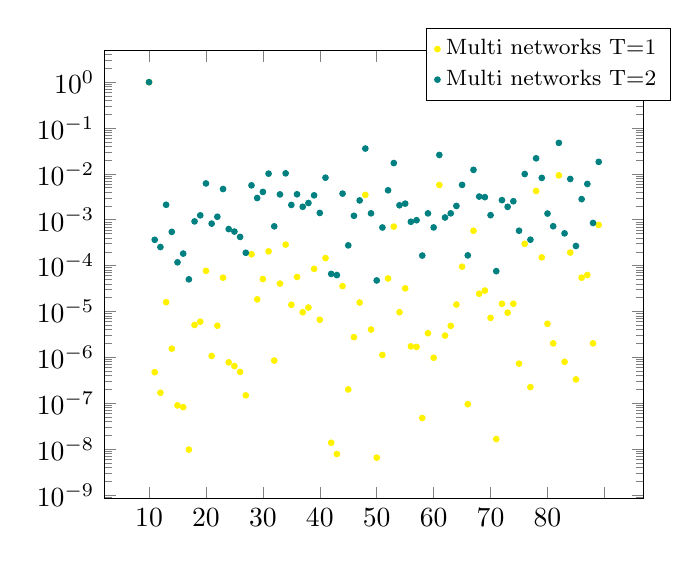
\begin{tikzpicture}
\begin{axis}[
    scatter/classes={
        t1={mark=*,mark size=1pt,yellow},
        t2={mark=*,mark size=1pt,teal}},
        xticklabels={0,10,...,80},
        max space between ticks=20,
        ymax=5,
        legend style={font=\footnotesize, at={(1.05,1.05)}, anchor=north east},
        ymode=log
]
\addplot[scatter,only marks,%
    scatter src=explicit symbolic]%
        table[meta=label] {
        x y label
        0 0.999996 t1
        1 4.74067748e-07 t1
        2 1.68915409e-07 t1
        3 1.59078106e-05 t1
        4 1.54497589e-06 t1
        5 8.94846783e-08 t1
        6 8.1939532e-08 t1
        7 9.73920698e-09 t1
        8 5.07651622e-06 t1
        9 5.99073371e-06 t1
        10 7.68106537e-05 t1
        11 1.0739685e-06 t1
        12 4.88770108e-06 t1
        13 5.45032883e-05 t1
        14 7.7609328e-07 t1
        15 6.45066687e-07 t1
        16 4.8090418e-07 t1
        17 1.48368015e-07 t1
        18 0.000176778308 t1
        19 1.83218663e-05 t1
        20 5.09219597e-05 t1
        21 0.000204199722 t1
        22 8.5038146e-07 t1
        23 4.05315051e-05 t1
        24 0.00028695356 t1
        25 1.39862685e-05 t1
        26 5.65815246e-05 t1
        27 9.60939336e-06 t1
        28 1.2160384e-05 t1
        29 8.49538999e-05 t1
        30 6.59140589e-06 t1
        31 0.000145837964 t1
        32 1.37212808e-08 t1
        33 7.7979943e-09 t1
        34 3.5759269e-05 t1
        35 1.9974649e-07 t1
        36 2.753256e-06 t1
        37 1.56400425e-05 t1
        38 0.0034847132 t1
        39 4.04186501e-06 t1
        40 6.49151768e-09 t1
        41 1.12618865e-06 t1
        42 5.23703504e-05 t1
        43 0.000708472565 t1
        44 9.643366e-06 t1
        45 3.19339277e-05 t1
        46 1.73286704e-06 t1
        47 1.68838706e-06 t1
        48 4.7516321e-08 t1
        49 3.35318e-06 t1
        50 9.789731e-07 t1
        51 0.00572819145 t1
        52 2.98230963e-06 t1
        53 4.85057838e-06 t1
        54 1.41581403e-05 t1
        55 9.46876886e-05 t1
        56 9.52081519e-08 t1
        57 0.000575062812 t1
        58 2.43306154e-05 t1
        59 2.85409725e-05 t1
        60 7.24742272e-06 t1
        61 1.64909248e-08 t1
        62 1.46882211e-05 t1
        63 9.40843568e-06 t1
        64 1.47085853e-05 t1
        65 7.28929861e-07 t1
        66 0.00029837051 t1
        67 2.2452188e-07 t1
        68 0.0042319329 t1
        69 0.000151225968 t1
        70 5.38985584e-06 t1
        71 2.0136951e-06 t1
        72 0.00927707274 t1
        73 7.97191274e-07 t1
        74 0.000192410018 t1
        75 3.30430738e-07 t1
        76 5.45635151e-05 t1
        77 6.2472028e-05 t1
        78 2.0144383e-06 t1
        79 0.000771420355 t1
        0 0.999371507 t2
        1 0.000365436097 t2
        2 0.000253972373 t2
        3 0.00211948766 t2
        4 0.000543583298 t2
        5 0.000117955943 t2
        6 0.000182778993 t2
        7 5.01304183e-05 t2
        8 0.000920311164 t2
        9 0.00124669599 t2
        10 0.00618139196 t2
        11 0.000821926347 t2
        12 0.00116133177 t2
        13 0.00467244204 t2
        14 0.000625254542 t2
        15 0.000551964047 t2
        16 0.000422341709 t2
        17 0.000190317197 t2
        18 0.00562379375 t2
        19 0.0029749202 t2
        20 0.00404134667 t2
        21 0.0101184616 t2
        22 0.000717772435 t2
        23 0.0035699357 t2
        24 0.0102657213 t2
        25 0.00210143235 t2
        26 0.00359309478 t2
        27 0.00191700673 t2
        28 0.0023164262 t2
        29 0.00340925869 t2
        30 0.00140511134 t2
        31 0.00825348977 t2
        32 6.58416127e-05 t2
        33 6.2191685e-05 t2
        34 0.00371531793 t2
        35 0.000276055932 t2
        36 0.00121954262 t2
        37 0.00263573568 t2
        38 0.0356703515 t2
        39 0.00137933754 t2
        40 4.74161971e-05 t2
        41 0.000677855775 t2
        42 0.00438557248 t2
        43 0.0172268308 t2
        44 0.00206874085 t2
        45 0.00224480671 t2
        46 0.000903137276 t2
        47 0.00097624566 t2
        48 0.000165608024 t2
        49 0.00137583978 t2
        50 0.000679590561 t2
        51 0.0258567065 t2
        52 0.00111949034 t2
        53 0.00137778866 t2
        54 0.00199883736 t2
        55 0.00574996961 t2
        56 0.00016704767 t2
        57 0.0122405603 t2
        58 0.0032009352 t2
        59 0.00310823884 t2
        60 0.00125794172 t2
        61 7.57119499e-05 t2
        62 0.00267555938 t2
        63 0.00191321619 t2
        64 0.00252913904 t2
        65 0.000575516912 t2
        66 0.00992801488 t2
        67 0.000366761713 t2
        68 0.0218409878 t2
        69 0.00817443028 t2
        70 0.00136213027 t2
        71 0.000721917394 t2
        72 0.0474319558 t2
        73 0.000504482056 t2
        74 0.00774006482 t2
        75 0.000267601464 t2
        76 0.00281227838 t2
        77 0.00602807713 t2
        78 0.0008496837 t2
        79 0.0182630532 t2
    };

    \addlegendentry{Multi networks T=1}
    \addlegendentry{Multi networks T=2}
\end{axis}
\end{tikzpicture}
\caption{The application of $T$ to the sigmoid function effectively reduces the amount of variance in the distribution of the multi networks targets.}
\label{100b}
\end{figure}

\begin{figure}
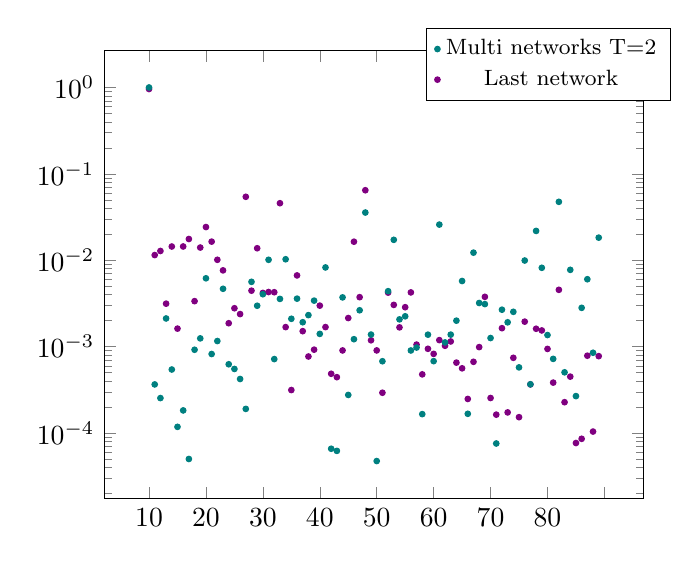
\begin{tikzpicture}
\begin{axis}[
    scatter/classes={
        t2={mark=*,mark size=1pt,teal},
        last={mark=*,mark size=1pt,violet}},
        xticklabels={0,10,...,80},
        max space between ticks=20,
        legend style={font=\footnotesize, at={(1.05,1.05)}, anchor=north east},
        ymode=log
]
\addplot[scatter,only marks,%
    scatter src=explicit symbolic]%
        table[meta=label] {
        x y label
        0 0.9588 last
        1 0.0114788624 last
        2 0.012801765 last
        3 0.003142994 last
        4 0.01441521 last
        5 0.0016169614 last
        6 0.01443137 last
        7 0.0176103535 last
        8 0.0033608385 last
        9 0.014026096 last
        10 0.02422393 last
        11 0.016426644 last
        12 0.0101222067 last
        13 0.007634055 last
        14 0.00186699215 last
        15 0.00278246115 last
        16 0.0023820986 last
        17 0.054223065 last
        18 0.004444426 last
        19 0.013769971 last
        20 0.0041849474 last
        21 0.00428614485 last
        22 0.004263856 last
        23 0.0457139095 last
        24 0.00168346805 last
        25 0.000314604945 last
        26 0.0066756575 last
        27 0.00151063205 last
        28 0.00076936535 last
        29 0.000922756035 last
        30 0.00298290475 last
        31 0.00168374 last
        32 0.00048524015 last
        33 0.00044354651 last
        34 0.0009040457 last
        35 0.0021433839 last
        36 0.0163847125 last
        37 0.003738416 last
        38 0.064595402 last
        39 0.00118486225 last
        40 0.00090440175 last
        41 0.000292819605 last
        42 0.00422010196 last
        43 0.00304306155 last
        44 0.0016717293 last
        45 0.0028602134 last
        46 0.00424374055 last
        47 0.0010562738 last
        48 0.000477810735 last
        49 0.0009441741 last
        50 0.000824641635 last
        51 0.0011900274 last
        52 0.0010229634 last
        53 0.00114778658 last
        54 0.000653365815 last
        55 0.000561440955 last
        56 0.00024805549 last
        57 0.00066774326 last
        58 0.0009878566 last
        59 0.0037700701 last
        60 0.000254453047 last
        61 0.000163284118 last
        62 0.00163621671 last
        63 0.000173378671 last
        64 0.000742614665 last
        65 0.0001527452 last
        66 0.00194739764 last
        67 0.000365420295 last
        68 0.00161086794 last
        69 0.00154027923 last
        70 0.000941527919 last
        71 0.00038372992 last
        72 0.0045468758 last
        73 0.000227520491 last
        74 0.000449689748 last
        75 7.66790656e-05 last
        76 8.57889861e-05 last
        77 0.000785611085 last
        78 0.000104022092 last
        79 0.000776493406 last
        0 0.999371507 t2
        1 0.000365436097 t2
        2 0.000253972373 t2
        3 0.00211948766 t2
        4 0.000543583298 t2
        5 0.000117955943 t2
        6 0.000182778993 t2
        7 5.01304183e-05 t2
        8 0.000920311164 t2
        9 0.00124669599 t2
        10 0.00618139196 t2
        11 0.000821926347 t2
        12 0.00116133177 t2
        13 0.00467244204 t2
        14 0.000625254542 t2
        15 0.000551964047 t2
        16 0.000422341709 t2
        17 0.000190317197 t2
        18 0.00562379375 t2
        19 0.0029749202 t2
        20 0.00404134667 t2
        21 0.0101184616 t2
        22 0.000717772435 t2
        23 0.0035699357 t2
        24 0.0102657213 t2
        25 0.00210143235 t2
        26 0.00359309478 t2
        27 0.00191700673 t2
        28 0.0023164262 t2
        29 0.00340925869 t2
        30 0.00140511134 t2
        31 0.00825348977 t2
        32 6.58416127e-05 t2
        33 6.2191685e-05 t2
        34 0.00371531793 t2
        35 0.000276055932 t2
        36 0.00121954262 t2
        37 0.00263573568 t2
        38 0.0356703515 t2
        39 0.00137933754 t2
        40 4.74161971e-05 t2
        41 0.000677855775 t2
        42 0.00438557248 t2
        43 0.0172268308 t2
        44 0.00206874085 t2
        45 0.00224480671 t2
        46 0.000903137276 t2
        47 0.00097624566 t2
        48 0.000165608024 t2
        49 0.00137583978 t2
        50 0.000679590561 t2
        51 0.0258567065 t2
        52 0.00111949034 t2
        53 0.00137778866 t2
        54 0.00199883736 t2
        55 0.00574996961 t2
        56 0.00016704767 t2
        57 0.0122405603 t2
        58 0.0032009352 t2
        59 0.00310823884 t2
        60 0.00125794172 t2
        61 7.57119499e-05 t2
        62 0.00267555938 t2
        63 0.00191321619 t2
        64 0.00252913904 t2
        65 0.000575516912 t2
        66 0.00992801488 t2
        67 0.000366761713 t2
        68 0.0218409878 t2
        69 0.00817443028 t2
        70 0.00136213027 t2
        71 0.000721917394 t2
        72 0.0474319558 t2
        73 0.000504482056 t2
        74 0.00774006482 t2
        75 0.000267601464 t2
        76 0.00281227838 t2
        77 0.00602807713 t2
        78 0.0008496837 t2
        79 0.0182630532 t2
    };

    \addlegendentry{Multi networks T=2}
    \addlegendentry{Last network}
\end{axis}
\end{tikzpicture}
\caption{Soften targets distribution still results more irregular than the one provided by last net policy, as these targets remains more precise.}
\label{100c}
\end{figure}

Using this approach, we record the scores given by the modified algorithm with respect to the ones given by iCaRL. We find that iCaRL outperforms our procedure by $1.2\%$ average incremental accuracy over the test set. A possible cause is that new distillation targets are characterized by very large variance with extremely low values, with probability distribution unevenly spreaded. The authors of \cite{hinton:2015} already studied this problem and its solution, which we applied to our case by adding a $T$ hyper-parameter in the sigmoid function (\ref{hinteq}), producing a soften targets distribution.
\begin{equation}
\sigma(x) = \frac{1}{1 + \exp(-x/T)} \label{hinteq}
\end{equation}
This is a modified sigmoid function which results in targets characterized by smaller deviation, as we show in Figure~\ref{100b}. We also jointly finetune the temperature $T$ and the learning rate, which we find to give better results at $T=2$ and learning rate equal to $3$.

\begin{table}
    \begin{center}
        \begin{tabular}{|r|c|}
        \hline
        Method & Avg. \\
        \hline\hline
        Last network (iCaRL) & $62.7\%$ \\
        Multi networks $T = 1$ & $61.1\%$ \\
        Multi networks $T = 2$ & $63.2\%$ \\
        \hline
        \end{tabular}
    \end{center}
\caption{Comparison of iCaRL accuracy scores with the modified algorithm using old nets distillation targets and temperature parameters in the sigmoid layer.}
\label{tab:3}
\end{table}

Accuracy scores on the test set are presented in Table~\ref{tab:3}. Figure~\ref{101} shows a comparison between our multi networks policy and the iCaRL baseline. We can observe a slight increase in accuracy due to the fact that we are giving more precise and meaningful targets to the distillation function. Moreover, the introduction of a temperature parameter $T$ in the sigmoid layer applied to old classes leads to an improvement.

\begin{figure}
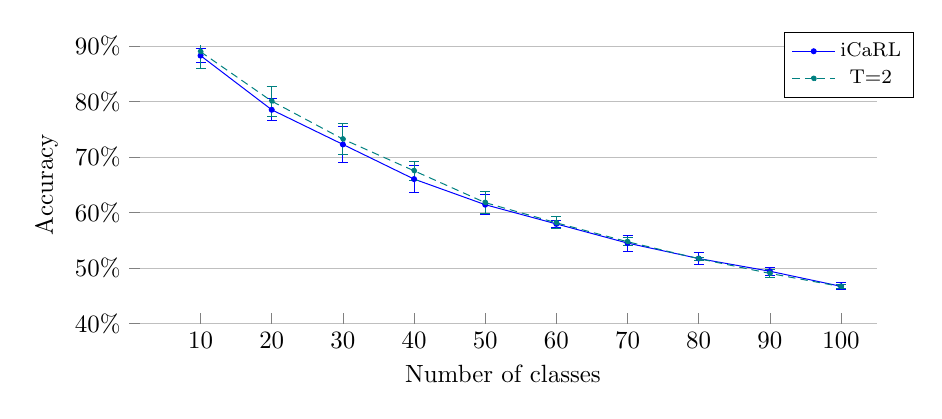
\begin{tikzpicture}[scale=0.9]
\begin{axis}[
        width=\columnwidth,
        height=5.5cm,
        axis line style={draw=none},
        xmin=0, xmax=105,
        xtick={10,20,...,100},
        tick pos=left,
        ymin=0.4, ymax=0.9,
        ytick={0.4,0.5,0.6,0.7,0.8,0.9},
        yticklabel={\pgfmathparse{\tick*100}\pgfmathprintnumber{\pgfmathresult}\%},
        point meta={y*100},
        xlabel=Number of classes,
        ylabel=Accuracy,
        legend style={font=\footnotesize, at={(1.05,1.05)}, anchor=north east},
        ymajorgrids=true
    ]

    % iCaRL scores
    \addplot+[
        blue,
        mark=*,
        mark options={scale=0.5},
        error bars/.cd,
            y fixed,
            y dir=both,
            y explicit,
            error bar style={solid}
    ] table [x=x, y=y,y error=error, col sep=comma] {
        x,  y,       error
        10, 0.88266667, 0.01228368,
        20, 0.78516667, 0.02002637,
        30, 0.72277778, 0.03299532,
        40, 0.66033333, 0.02372967,
        50, 0.61426667, 0.0181272,
        60, 0.57961111, 0.00563773,
        70, 0.54514286, 0.01427571,
        80, 0.51729167, 0.01019923,
        90, 0.49444444, 0.00730353,
        100, 0.46723333, 0.00642512
    };

    % custom loss
    \addplot+[
        teal,
        densely dashed,
        mark=*,
        mark options={scale=0.5},
        error bars/.cd,
            y fixed,
            y dir=both,
            y explicit,
            error bar style={solid}
    ] table [x=x, y=y,y error=error, col sep=comma] {
        x,  y,       error
        10, 0.88966667, 0.03007029,
        20, 0.80066667, 0.02723458,
        30, 0.73233333, 0.02779821,
        40, 0.67533333, 0.01736056,
        50, 0.618, 0.01940515,
        60, 0.58161111, 0.01076374,
        70, 0.54752381, 0.00705887,
        80, 0.51709167, 0.00251001,
        90, 0.49051852, 0.007267,
        100, 0.46676667, 0.00334896
    };
    \addlegendentry{iCaRL}
    \addlegendentry{T=2}
\end{axis}
\end{tikzpicture}
\caption{Incremental accuracy over the test with distillation targets obtained with multi net approach. $T$ is set to $2$ while the learning rate is equal to $2$. Our new proposed approach outperforms iCaRL by $0.5\%$ of incremental average accuracy.}
\label{101}
\end{figure}

\subsection{Features Representation Drift Study}
\label{frds}
In the incremental learning protocol, we assume that only a fixed amount of data from the old classes is stored, in order to maintain the memory footprint bounded. As a consequence, training steps are performed over unbalanced class distributions. One way to address this problem is to use a knowledge distillation loss. We think that another interesting way of tackling this issue is to try to maintain as much as possible a similar feature representation between the network at step $N-1$ and the one at step $N$. In order to do this, we shift our focus to the outputs of the last layer of the feature extractor, which is used to classify images at test time. Firstly, we demostrate the existence of a residual features representation drift. Then, we propose an approach that tries to limit it.

To classify unseen data, iCaRL computes the mean of exemplars for all known classes. At the end of each incremental learning step, we store the class prototypes, which we suppose are representative of the features learned by the network. At step $N$ we compare the prototypes of the network with those learned at step $N-1$. The difference defining the drift is computed as mean square error (MSE) between all $64$ entries of the mean of exemplars vectors. These $64$ entries correspond to the output nodes of our feature extractor. All entries are weighted by a coefficient, defined for each label, which states the importance of a feature for that specific class, since we are only interested in avoiding drift of meaningful features (see Appendix~\ref{appendix}).

\begin{figure}
\begin{center}
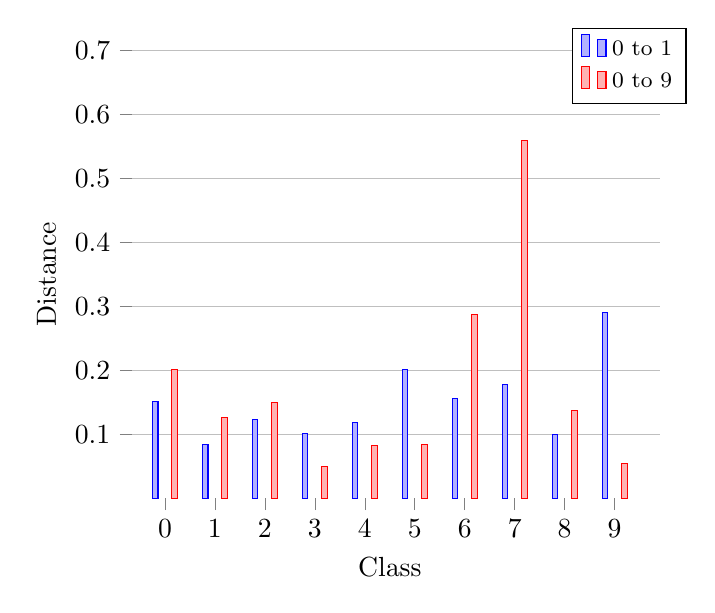
\begin{tikzpicture}
\begin{axis}[
        % every axis plot post/.style={/pgf/number format/fixed},
        ybar=5pt,
        bar width=2pt,
        ymin=0,
        ymax=0.7,
        % symbolic x coords={0,1,2,3,4,5,6,7,8,9},
        xtick={0,1,2,3,4,5,6,7,8,9},
        ytick={0.1,0.2,...,0.7},
        axis line style={draw=none},
        tick pos=left,
        xlabel=Class,
        ylabel=Distance,
        legend style={font=\footnotesize, at={(1.05,1.05)}, anchor=north east},
        ymajorgrids=true
    ]
    \addplot coordinates {(0,0.1515) (1,0.0844) (2,0.1231) (3,0.1016) (4,0.1191) (5,0.2006) (6,0.1563) (7,0.1776) (8,0.0996) (9,0.2898)};
    \addplot coordinates {(0,0.2019) (1,0.1269) (2,0.1491) (3,0.0497) (4,0.0824) (5,0.0842) (6,0.2873) (7,0.5583) (8,0.1366) (9,0.0540)};
    \addlegendentry{0 to 1}
    \addlegendentry{0 to 9}
\end{axis}
\end{tikzpicture}
\end{center}
\caption{Weighted MSE drift from step 0 to 1 and 0 to 9. Inspecting the results, we confirm the features representation drift hypothesis. Moreover, we observe how the drift not only propagates, but also amplifies from step 1 to 9.}
\label{5:histogram}
\end{figure}

In Figure~\ref{5:histogram} we show the drift between the representation learned at step 0 versus those learned at step 1 and 9. We can observe significant error between two consecutive steps, and we can also see that it propagates and increases over the networks.

To mitigate the drift, we add a contribution to the loss which tries to minimize the distance between important features. We choose a smooth L1 loss function (\ref{eq:smoothl1}) weighted by a parameter $\alpha$ which defines the importance of this contribution:
\begin{equation}
\text{loss}(x, y) = \frac{1}{n} \sum_{l} z_{l}*\alpha \label{eq:smoothl1}
\end{equation}
\[
    z_{i} =
    \begin{cases}
    0.5 (x_i - y_l)^2, & \text{if } |x_i - y_l| < 1 \\
    |x_i - y_l| - 0.5, & \text{otherwise }
    \end{cases}
\]
where $x_{i}$ is L2 normalized feature representation of image $i$ of the trained network, while target $y_{l}$ is the last network prototype corresponding to label $l$. $\alpha$ is an hyper-parameter to be tuned along with the learning rate.
This loss behaves as L2 if the it falls below $1$, and as L1 otherwise.

We jointly tune $\alpha$ and the initial learning rate, which we set to $10^{-4}$ and $0.3$ respectively. We train the network for $80$ epochs, and decrease the initial learning rate by a factor of $5$ after $75$ epochs.

\begin{figure}
\begin{center}
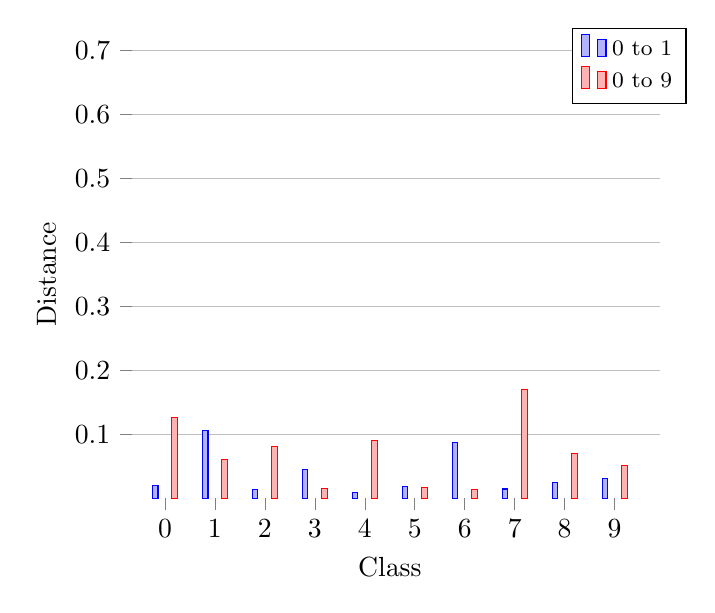
\begin{tikzpicture}
\begin{axis}[
        % every axis plot post/.style={/pgf/number format/fixed},
        ybar=5pt,
        bar width=2pt,
        ymin=0,
        ymax=0.7,
        % symbolic x coords={0,1,2,3,4,5,6,7,8,9},
        xtick={0,1,2,3,4,5,6,7,8,9},
        ytick={0.1,0.2,...,0.7},
        axis line style={draw=none},
        tick pos=left,
        xlabel=Class,
        ylabel=Distance,
        legend style={font=\footnotesize, at={(1.05,1.05)}, anchor=north east},
        ymajorgrids=true
    ]
    \addplot coordinates {(0,0.0207) (1,0.1064) (2,0.0145) (3,0.0449) (4,0.0098) (5,0.0190) (6,0.0872) (7,0.0147) (8,0.0248) (9,0.0315)};
    \addplot coordinates {(0,0.1261) (1,0.0603) (2,0.0804) (3,0.0151) (4,0.0906) (5,0.0173) (6,0.0138) (7,0.1703) (8,0.0702) (9,0.0517)};
    \addlegendentry{0 to 1}
    \addlegendentry{0 to 9}
\end{axis}
\end{tikzpicture}
\end{center}
\caption{Drift reduction from net 0 to 1 and 0 to 9, comparing features representation with and without smooth L1 loss contribute over the last layer of the feature extractor.}
\label{5:histogram2}
\end{figure}

In Figure~\ref{5:histogram2} we can quantitatively observe how the loss contribution that we introduced is able to mitigate drift over features. The adopted measure is effective, but results in a drop of accuracy over the incremental training steps, as we can see in Figure~\ref{105}. This can be explained by the fact that without properly balancing the selected hyper-parameters, preventing the drift also means preventing an effective learning. Nevertheless, we consider this a promising procedure, since the model may produce a more general feature representation, trying to balance with the learning and distillation needs. Despite this, due to lack of time and computational resources, we are not able to explore the problem any further.

\begin{figure}
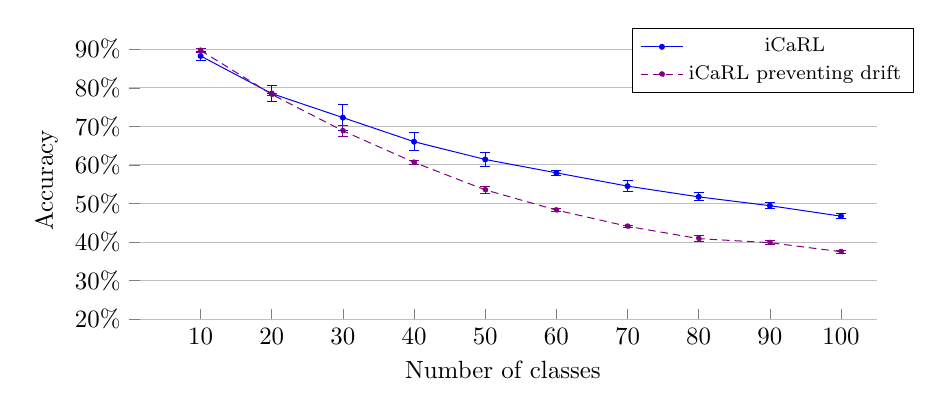
\begin{tikzpicture}[scale=0.9]
\begin{axis}[
        width=\columnwidth,
        height=5.5cm,
        axis line style={draw=none},
        xmin=0, xmax=105,
        xtick={10,20,...,100},
        tick pos=left,
        ymin=0.2, ymax=0.92,
        ytick={0.2,0.3,0.4,0.5,0.6,0.7,0.8,0.9},
        yticklabel={\pgfmathparse{\tick*100}\pgfmathprintnumber{\pgfmathresult}\%},
        point meta={y*100},
        xlabel=Number of classes,
        ylabel=Accuracy,
        legend style={font=\footnotesize, at={(1.05,1.05)}, anchor=north east},
        ymajorgrids=true
    ]

    % iCaRL scores
    \addplot+[
        blue,
        mark=*,
        mark options={scale=0.5},
        error bars/.cd,
            y fixed,
            y dir=both,
            y explicit,
            error bar style={solid}
    ] table [x=x, y=y,y error=error, col sep=comma] {
        x,  y,       error
        10, 0.88266667, 0.01228368,
        20, 0.78516667, 0.02002637,
        30, 0.72277778, 0.03299532,
        40, 0.66033333, 0.02372967,
        50, 0.61426667, 0.0181272,
        60, 0.57961111, 0.00563773,
        70, 0.54514286, 0.01427571,
        80, 0.51729167, 0.01019923,
        90, 0.49444444, 0.00730353,
        100, 0.46723333, 0.00642512
    };

    \addplot+[
        violet,
        densely dashed,
        mark=*,
        mark options={scale=0.5},
        error bars/.cd,
            y fixed,
            y dir=both,
            y explicit,
            error bar style={solid}
    ] table [x=x, y=y,y error=error, col sep=comma] {
        x,  y,       error
        10, 0.897   ,0.005
        20, 0.783   ,0.003
        30, 0.6885  ,0.0145
        40, 0.60675 ,0.00425
        50, 0.5355  ,0.0095
        60, 0.483   ,0.004
        70, 0.441   ,0.003
        80, 0.409   ,0.008
        90, 0.3985  ,0.0045
        100, 0.375   ,0.004
    };
    \addlegendentry{iCaRL}
    \addlegendentry{iCaRL preventing drift}
\end{axis}
\end{tikzpicture}
\caption{iCaRL scores with feature drift distillaton loss term. Compared to the plain iCaRL framework, our implementation leads to worse incremental accuracy. This is because of the additional loss contribute that, while preserving the old representation, also prevents the network from adequately learning the new task.}
\label{105}
\end{figure}

\begin{figure*}
\begin{center}
\begin{subfigure}{0.48\textwidth}
    \begin{tikzpicture}
    \begin{axis}[
        scatter/classes={
            p_0={mark=triangle*,red},
            p_1={mark=triangle*,green},
            p_2={mark=triangle*,blue},
            p_3={mark=triangle*,cyan},
            p_4={mark=triangle*,orange},
            p_5={mark=triangle*,yellow},
            p_6={mark=triangle*,lime},
            p_7={mark=triangle*,olive},
            p_8={mark=triangle*,purple},
            p_9={mark=triangle*,violet},
            0={mark=*,mark size=0.1pt,red},
            1={mark=*,mark size=0.1pt,green},
            2={mark=*,mark size=0.1pt,blue},
            3={mark=*,mark size=0.1pt,cyan},
            4={mark=*,mark size=0.1pt,orange},
            5={mark=*,mark size=0.1pt,yellow},
            6={mark=*,mark size=0.1pt,lime},
            7={mark=*,mark size=0.1pt,olive},
            8={mark=*,mark size=0.1pt,purple},
            9={mark=*,mark size=0.1pt,violet}},
            yticklabels={,,},
            xticklabels={,,},
            axis line style={draw=none},
            tick style={draw=none}
    ]
        % ymode=log]
    \addplot[scatter,only marks,%
        scatter src=explicit symbolic]%
            table[meta=label] {
            x y label
            -118.606094 -0.21710598 p_0
            -87.08352 98.89436 p_1
            11.943616 101.563995 p_2
            81.558624 -49.63411 p_3
            13.321995 -110.08728 p_4
            -88.96968 -87.52829 p_5
            -25.26445 -40.51796 p_6
            -43.917824 34.04424 p_7
            96.29411 53.890877 p_8
            29.878693 12.830559 p_9
            -33.40482 15.0145855 1
            16.19252 -21.838076 3
            -25.785852 -12.714153 2
            -6.858647 -11.693158 3
            -24.542824 -9.615482 2
            -31.604956 14.5274 1
            -23.350792 -9.671894 2
            -0.56374216 -15.240189 5
            -25.701233 -7.7017817 2
            0.8942476 20.960304 6
            2.3480465 -0.0045972406 7
            -20.821573 -12.381163 2
            16.840725 -22.156874 3
            14.158617 -20.526993 3
            -2.9924824 -12.771622 5
            -3.4880986 -15.529737 5
            -31.031492 15.054776 1
            -31.074953 10.587577 1
            6.904706 -1.2406994 7
            10.363907 14.634178 8
            -32.647038 14.500011 1
            6.395078 0.7784343 9
            -15.989792 -3.7064936 2
            18.756973 -23.021503 3
            17.93953 3.2188056 0
            -0.4556984 -13.126831 5
            -1.9282008 22.756351 6
            12.62206 -8.195475 9
            21.667953 1.6033002 0
            0.47092253 -2.458082 7
            20.183418 1.0328051 0
            -26.979193 -8.818688 4
            -2.4061067 -4.282065 4
            18.012102 4.635099 0
            0.3796521 -3.228855 5
            17.81381 -23.188314 3
            -27.416962 -8.763058 2
            -27.21014 -10.512572 2
            16.329468 -22.247541 3
            -24.873394 -9.970688 2
            20.916767 4.5590487 4
            0.4729589 -0.70833415 7
            13.154982 -19.242447 3
            17.589983 -19.018835 3
            2.6811578 2.6778033 7
            11.015476 -4.575108 9
            -24.172445 -8.9989395 2
            -1.4684336 20.47025 6
            17.989437 2.8619685 0
            -3.2778397 -12.766013 5
            1.4786327 2.3796463 7
            10.538985 14.251024 8
            -2.044413 22.777794 6
            1.9287703 -2.8264554 7
            14.42354 -23.887388 3
            -28.891975 15.685429 1
            -23.553616 -10.397527 2
            -4.8379207 21.38883 6
            -33.6875 13.003334 1
            -24.978592 -9.760761 2
            -17.298077 -0.93284094 4
            16.5597 5.9017925 7
            19.994827 2.8753426 0
            -32.49064 14.634235 1
            18.87742 0.09781251 0
            -2.7725945 -13.557329 5
            -2.7992253 23.578747 6
            -2.8209095 24.89438 6
            -30.160658 15.274891 1
            8.263823 12.308038 8
            5.3970475 11.8864 8
            -21.916485 -9.799106 4
            8.886431 -5.7568374 9
            -5.1070623 -15.987507 5
            -2.835603 -16.06672 5
            -30.267061 13.319094 1
            18.671484 -21.934675 3
            18.930147 -22.420979 3
            12.604058 -5.053461 9
            16.874935 -22.562637 3
            -32.44897 15.697679 1
            15.665721 -21.761847 3
            -33.065155 16.629734 1
            17.806953 -22.289827 3
            -4.4896464 -16.221418 5
            20.697424 5.834038 3
            -1.6346647 24.253378 6
            -18.030132 -1.5171281 4
            9.408201 12.545824 8
            20.109318 -0.32293677 0
            18.37061 1.8721632 0
            17.186686 -21.584671 3
            -1.317549 23.222832 6
            -3.3610518 -16.104177 5
            -27.40919 -11.057074 2
            10.764113 -5.615246 9
            -23.222326 -7.783978 4
            -0.59512806 -13.570926 5
            8.158934 12.68297 8
            17.619854 2.0987742 0
            15.589902 -18.59256 3
            -3.7518494 25.974363 6
            -31.278635 13.823401 1
            19.32656 3.4516628 0
            -15.688529 -0.59376854 4
            18.984713 1.7622645 0
            -6.5668426 -9.916363 4
            -30.776583 12.054362 1
            7.7225356 8.5142 8
            14.668388 0.9007969 0
            -20.958618 -9.078095 2
            -3.3441215 22.98267 6
            7.639886 9.728045 8
            -4.4277973 -16.57095 5
            16.164011 -20.031075 3
            9.7328005 14.46562 8
            -33.196404 13.375091 1
            -19.466972 -1.616774 5
            7.332616 13.173264 8
            -24.208313 -10.175905 2
            12.7210455 -5.680454 9
            -3.5167143 -15.781541 5
            -33.732536 15.57796 1
            4.1524954 2.2440975 7
            -0.12642862 0.3019202 7
            0.28134993 21.066168 6
            9.81371 13.864463 8
            5.162347 2.6211615 7
            -12.420894 0.9646151 4
            8.735592 11.961415 8
            -3.2154198 21.099495 6
            -2.548036 24.455902 6
            19.258 0.7187419 0
            -35.577026 15.380676 6
            -3.5701377 19.598852 6
            -32.06182 14.99366 1
            0.043354638 22.091137 6
            -29.777231 11.485829 1
            -28.256674 15.87279 7
            -31.831295 14.06103 1
            -12.910118 -0.22481698 4
            -6.243642 -15.675293 5
            10.305365 13.391506 8
            18.080166 3.549371 0
            19.632578 1.7661165 0
            -15.402152 0.09608479 4
            -23.464836 -10.982004 2
            14.806321 -2.1061459 0
            16.589994 -0.39155552 0
            -27.418356 -9.698774 2
            -17.822603 2.5781996 4
            12.381824 -6.9357924 9
            20.256498 2.6398535 0
            1.3331835 0.64017373 7
            5.9099755 2.874276 2
            17.042269 -20.781967 3
            10.433901 14.647145 8
            -14.655142 -0.75167847 4
            -3.1100068 25.50561 6
            -24.959206 -10.53096 2
            -24.169004 -10.995882 2
            2.5623033 2.8722708 7
            18.703232 3.9425192 0
            -2.880615 25.605808 6
            11.913833 -7.812142 9
            4.2923493 0.93281174 9
            -14.461689 -2.0391743 4
            -13.890312 -2.4522943 4
            20.829031 2.2685134 0
            -15.672896 0.7760173 4
            19.23592 0.059547916 0
            -24.26728 -8.458528 2
            -3.8799844 23.04252 6
            15.01284 7.6192145 0
            -1.8316987 -14.177269 5
            -3.0074658 -14.591267 5
            -28.396856 12.278922 1
            -27.696178 -7.7608166 2
            6.5001287 4.0240297 2
            -16.97343 -2.6344984 2
            -3.30116 -14.475946 5
            -28.605537 13.736934 1
            4.226381 -1.8938969 7
            -16.380316 -0.85064405 4
            14.545644 -18.18387 9
            -3.2855644 11.844837 6
            17.364876 -21.711117 3
            4.385362 -3.8188546 3
            0.4381778 -0.94089395 7
            -32.268234 12.318268 1
            8.421879 13.191986 8
            -24.092491 -9.563997 2
            11.115081 -5.472408 9
            -2.40506 -15.365094 5
            -23.408175 -13.100308 2
            -24.309647 -13.005181 2
            19.387257 1.2833987 0
            7.4702406 -2.9092999 0
            -26.624195 -9.231494 2
            -24.802994 -11.7122 2
            -18.053623 -2.08006 4
            15.372259 -23.82729 3
            1.6757782 4.365583 7
            9.69277 -5.3698134 9
            -0.23038113 3.3218117 7
            -18.949062 0.33864754 4
            -28.430437 13.0892 1
            -23.134264 -11.737393 2
            17.566368 -21.9148 3
            15.696326 1.4179419 7
            -25.072046 -11.219999 2
            13.825644 3.470373 0
            21.717222 1.675108 0
            -32.082394 17.15113 1
            1.5709207 1.1682389 7
            1.1093465 5.981563 7
            -23.360552 -9.14355 2
            -4.3076506 23.507584 6
            7.5645056 12.581176 8
            -27.3745 -9.412629 2
            6.307044 -2.0330708 9
            9.66192 -7.2910075 5
            6.9289465 -1.1789753 7
            12.516217 1.4188336 0
            -2.2634914 -13.573259 5
            1.883205 -0.38920462 7
            -2.2217207 21.832676 6
            5.7741814 7.8984985 4
            -29.129442 13.13652 1
            8.485478 -2.6622279 9
            14.196844 -20.83092 3
            -25.928152 -9.316882 2
            -31.253464 14.576414 1
            -33.438213 15.051057 1
            18.37036 -21.585014 3
            7.57079 11.950116 8
            -2.779671 -15.042027 5
            -3.1002877 22.581976 6
            1.553942 1.7698628 7
            -3.9503994 -13.802179 5
            -0.874912 0.82678914 7
            -1.792339 23.625319 6
            1.4280931 2.381901 7
            9.952006 -2.5281904 3
            -2.8858786 25.265629 6
            -22.437735 -12.312443 2
            10.165556 12.662812 8
            -3.7960672 22.325523 6
            -2.4902527 -15.553435 5
            12.231805 -4.8615427 9
            19.742346 0.45823547 0
            15.002719 -4.8023 9
            -18.971008 -1.9597623 4
            0.008457499 22.02283 6
            6.926387 14.176923 7
            16.721237 -21.020988 3
            16.686747 -21.167486 3
            14.890887 -4.9922366 9
            -1.0889971 2.6380966 7
            8.3464 12.794401 8
            -25.419458 -9.111247 2
            19.217028 0.95917577 0
            17.420717 -21.011425 3
            2.3814285 -0.66817933 7
            9.592626 -6.7944407 9
            -21.509176 -10.980022 2
            -2.7836185 24.58857 6
            -2.9862814 26.63889 6
            -4.1411805 -15.7659855 5
            -22.83814 -10.028729 2
            -0.19405001 -9.165824 7
            12.597122 -7.559046 9
            14.952339 -25.073473 3
            17.248531 -23.271418 3
            9.423733 -8.082771 9
            -33.39096 14.36028 1
            15.881372 -23.087908 3
            9.300279 8.469769 8
            -24.742996 -8.229014 2
            -27.612436 12.83475 7
            -4.081206 -15.802828 5
            -25.013145 -9.071339 2
            8.976926 13.60628 8
            -26.928019 -9.519039 2
            6.42617 13.962435 8
            16.25769 -19.85805 3
            0.6746978 1.3720124 7
            15.509914 -23.417292 3
            -17.956196 -2.2027886 4
            -16.00774 -1.2228417 4
            -5.263166 -15.617576 5
            9.411544 13.229384 8
            11.835108 -6.302904 9
            -6.005211 -14.762452 5
            -4.03162 -16.065414 5
            16.409922 -24.136133 3
            -25.841227 -9.570212 2
            5.4850926 -1.7019023 7
            -21.227123 -12.184083 2
            -1.3334364 -1.3707829 7
            -0.37032422 -15.036986 9
            19.24744 4.3448052 0
            1.675789 -2.5515594 7
            12.9528265 -5.3159175 9
            -1.2929708 3.1745539 7
            9.30795 13.789665 8
            18.92415 3.1678178 0
            -5.288914 22.831518 6
            -13.064861 -0.80576605 4
            -3.9398146 24.838257 6
            -3.3572311 -13.870565 5
            -23.837729 -9.078087 2
            -0.8390419 -8.8602705 9
            -5.3374753 23.25507 6
            14.594052 -21.85054 3
            -28.810837 15.955724 1
            10.421788 -6.187332 9
            -28.367311 -11.497836 2
            2.2255828 5.5170555 7
            -26.993313 -10.854426 2
            -32.0633 16.535086 1
            15.291766 -19.186245 3
            -3.248921 25.086456 6
            -2.8137827 20.01301 6
            19.265545 1.056649 0
            1.6022398 -1.2413129 7
            16.790144 -21.58989 3
            -2.1005924 23.528524 6
            -6.7836123 -15.012533 5
            13.3807535 0.368271 7
            2.2689686 1.1691251 7
            19.706293 4.607921 0
            -0.27330092 19.06946 6
            20.309244 2.0081422 0
            10.31658 -7.614902 9
            -26.000387 -10.165485 2
            7.399565 11.241082 8
            -14.419157 1.3316422 1
            -17.350285 1.511971 4
            18.460114 2.1800086 0
            -2.54122 -14.702064 5
            17.414547 -23.07805 3
            -1.6280714 3.8225431 7
            0.5354383 20.648209 6
            7.354815 12.623519 8
            16.227823 2.8029184 0
            -33.686134 13.984021 1
            -15.980598 -0.699493 4
            16.065184 -24.201883 3
            -3.4906085 -16.196716 5
            9.10987 14.814099 8
            -5.4113073 -16.580603 5
            -2.2406785 24.617126 6
            6.814666 12.17971 8
            -33.20639 14.470723 1
            -1.0151807 -10.578302 5
            4.707064 -1.39293 7
            -4.2643647 -15.2323675 5
            -19.150942 -3.2855568 2
            17.70586 5.0081654 0
            5.72508 -1.7234704 7
            4.1464458 -0.33859196 7
            -26.567085 -9.113104 2
            5.933079 10.418409 8
            -5.4098396 -15.642995 5
            -15.4212885 -3.7157772 2
            -2.3966734 22.936117 6
            8.228606 -0.5632686 8
            3.599879 4.336787 7
            10.867509 -8.455145 9
            14.975272 -20.670874 3
            18.036947 4.309251 0
            9.769934 11.968467 8
            13.820643 -22.13367 3
            -33.487736 14.251983 1
            9.684552 13.582235 8
            11.243755 -6.370539 9
            -16.617052 0.6940581 4
            12.203214 -8.095737 9
            1.3506682 0.845872 7
            -1.4237643 21.349781 6
            10.435461 2.0213764 5
            -2.8251765 -14.464585 5
            18.026606 5.754714 0
            10.728374 9.918592 3
            16.981836 -23.483137 3
            8.856704 11.835578 8
            -33.79594 14.626492 1
            -30.930882 15.236077 1
            -17.600319 -3.7648842 4
            -26.604696 -8.254871 2
            12.90043 -7.429657 9
            -2.7021098 22.182377 6
            1.4906195 -4.975985 5
            11.839906 -4.3518853 9
            -4.005511 23.448425 6
            9.872772 16.078054 8
            9.102126 12.172929 8
            -16.199339 -0.83511764 4
            10.603216 -9.086744 9
            -2.8103333 22.825907 6
            7.793502 15.92294 8
            -24.398596 -12.384817 2
            -22.84295 -12.199618 7
            -2.7604606 27.117315 6
            -15.61258 -0.23700657 4
            -25.16272 -9.624443 2
            -11.75155 1.041162 4
            -3.8180237 24.02703 6
            -32.679153 11.446842 1
            -2.618984 -4.317482 4
            9.854437 -6.520456 9
            15.020241 7.4596386 0
            20.773752 4.1445765 0
            0.38446784 0.6457535 7
            16.951183 7.601377 0
            -32.543304 13.882397 1
            -13.795448 -3.6165683 4
            18.162632 -21.6292 3
            -30.04662 13.932047 1
            -0.86793417 -10.037466 5
            -16.903238 -0.4642302 4
            17.377142 -21.542866 3
            11.760613 -7.170744 9
            -3.90885 25.140171 6
            0.74317217 6.068759 4
            -32.86389 13.42345 1
            -33.18423 15.006296 1
            11.886252 -8.935477 9
            18.89892 -21.705555 3
            11.877731 -4.694028 9
            5.388823 3.0786297 7
            21.219366 2.5994055 0
            9.932554 13.379403 8
            21.254257 2.999288 0
            -26.673532 -9.878823 2
            19.248377 1.097004 0
            13.584762 -6.25852 9
            1.7077883 0.8031279 7
            -26.906591 15.901908 6
            -2.3986561 26.998907 6
            12.954336 -5.199506 9
            -5.1056237 24.183727 6
            -4.984494 21.120121 6
            17.438105 -23.106014 3
            9.486391 -7.282656 9
            -5.243735 22.029282 6
            16.698448 -23.61091 3
            3.1742585 2.1822677 7
            3.0963318 -0.5214096 9
            7.7641487 9.205924 8
            -24.359695 -11.728707 2
            12.698979 -6.2429695 9
            -23.246815 -12.696159 2
            16.22345 -21.393158 3
            6.8107085 -5.6685605 9
            18.220503 -23.572855 3
            10.502016 11.886537 8
            -17.768106 -2.5282025 4
            -5.7185383 25.489054 6
            -22.55865 -10.273927 2
            -34.031975 14.470293 1
            17.685802 1.1331962 0
            16.728827 0.21727304 0
            11.690912 -6.8090806 9
            11.896736 -7.1383634 9
            11.799693 1.8596877 0
            -26.501968 -7.402526 2
            -17.367632 -0.46349 4
            19.819515 3.5536869 0
            0.98633444 19.965044 6
            18.61754 2.783843 0
            -27.285131 -8.349743 2
            18.090857 -21.368143 3
            -14.836209 -2.6592627 4
            14.960611 -23.544369 3
            6.9101553 -2.1314468 9
            -32.106037 14.78365 1
            6.7938075 12.53464 8
            11.596745 -6.806962 9
            8.443867 13.63527 8
            6.8777094 13.960866 8
            1.4906504 -0.06861594 7
            -15.691276 -0.76791865 4
            0.9898153 2.524026 7
            -31.352839 11.011025 1
            -17.009096 -0.84143484 4
            -6.7155385 -10.34302 5
            17.259157 -23.351408 3
            -28.628721 13.186428 1
            0.8104619 0.42599222 9
            -17.40092 -0.50162375 4
            -32.401722 13.649932 1
            20.976677 2.56101 0
            20.45988 1.1413795 4
            -3.1377358 23.817995 6
            -4.0845923 -14.939709 5
            5.869625 1.6790713 7
            20.55019 1.377027 0
            -3.6082752 21.384624 6
            18.902868 1.9757979 0
            -2.8304057 24.502071 6
            15.6750145 -22.664303 3
            -34.729424 14.489255 1
            -26.010054 -9.37978 2
            13.286372 -7.566592 9
            10.788757 -6.388174 9
            -4.057935 -11.342541 5
            -4.472256 20.712341 6
            -13.258818 0.4943961 4
            20.255709 4.439072 0
            6.8069963 -5.826614 9
            13.053888 -7.805555 9
            -33.578976 15.914795 1
            12.139751 -7.090634 9
            -26.489965 -9.099851 2
            9.352176 -9.695949 8
            -25.791424 -7.1768913 2
            9.677464 1.5202574 8
            9.722403 14.541073 8
            -24.876734 -9.626255 2
            12.51519 -9.460221 9
            8.207228 13.449522 8
            9.099785 -7.1975946 9
            9.85209 13.998195 8
            5.559004 1.6275486 7
            10.5228405 -3.4012995 9
            -33.31391 14.471031 1
            13.4507 -5.9584455 9
            14.566214 7.7821465 3
            17.696573 3.2842784 0
            -25.599628 -10.155855 2
            -26.237959 -8.701055 2
            -25.089106 -10.630259 2
            -18.608189 -1.2783722 4
            3.8506346 1.5333087 7
            12.221167 -7.148569 9
            4.9285517 -3.3847764 4
            -3.7270753 24.802458 6
            -16.72854 -1.9463224 4
            -14.729077 1.1274835 4
            12.056883 -7.4020705 9
            5.374368 -5.62021 5
            1.9389728 0.9453085 7
            16.784986 -21.287193 3
            16.980297 2.1544456 0
            13.752553 -20.669777 3
            9.914632 10.681833 8
            20.285011 3.0542076 0
            19.859879 1.6250135 0
            -2.7655396 25.395939 6
            16.813128 -23.822958 3
            15.937507 2.1256258 0
            -3.5900671 -13.766149 5
            -1.8495892 4.283633 4
            -21.588188 -9.852139 4
            -30.086641 12.494538 1
            15.084567 -18.617012 3
            -3.8706338 -11.400367 5
            2.5409408 0.6420512 7
            -32.87963 14.037158 1
            9.969559 12.218312 8
            5.8531137 16.31347 6
            10.251209 -8.2966795 9
            16.737295 -22.543566 3
            -7.253256 -14.632556 5
            6.024988 16.225807 8
            -5.3185883 23.827599 6
            3.661262 4.15566 7
            3.437365 -3.0247705 3
            7.5682125 10.433903 8
            8.186908 12.79438 8
            -0.121980846 -0.6000107 7
            -23.368568 -6.890635 2
            18.417679 4.3526607 0
            -32.857212 11.024732 1
            -14.803765 0.25407925 4
            -0.11662878 22.496702 6
            -31.709496 12.467468 1
            5.8355265 -1.6521785 7
            0.92925376 -2.1592772 7
            15.567802 -20.833902 3
            17.940096 0.20584099 9
            5.2955317 12.443905 8
            -34.304424 15.113003 1
            10.2790575 14.711073 8
            -22.325853 -9.104092 2
            15.38167 -21.602654 3
            7.080892 10.453763 8
            -2.5588055 -11.99792 5
            -4.118229 -12.33369 5
            -2.7027106 -14.108852 5
            16.686874 4.786215 0
            14.382063 -20.830725 3
            -25.924082 -9.694097 2
            8.730075 -3.7107887 7
            16.444841 -25.582916 3
            -2.3875575 -14.397446 5
            18.467695 4.1023326 0
            -2.78671 21.593021 6
            -3.8521316 23.112326 6
            -15.877012 -1.7519643 4
            -13.3861475 -0.25822547 4
            18.146803 3.8636398 0
            -11.971246 -0.74643487 4
            -5.978454 -14.540598 5
            -15.67597 -2.6650221 4
            10.297417 3.996669 3
            -30.613049 11.111015 1
            -31.217873 15.982736 1
            -14.631879 0.31036544 4
            11.891472 -2.3299668 2
            17.13487 -22.231941 3
            11.205 -4.483746 9
            15.405123 -21.955223 3
            -0.967093 0.02346513 7
            12.669181 -5.542949 9
            17.524355 2.8366103 0
            -1.6449789 3.0273092 7
            -4.2817755 22.549597 6
            -3.6881733 24.09869 6
            -0.5582076 3.377711 7
            -3.2218552 24.08998 6
            18.922382 3.9405818 0
            -25.917665 -10.89629 2
            11.134765 -5.9180512 9
            -32.079514 15.261401 1
            4.818782 5.1825843 7
            9.865944 16.190458 8
            8.318647 11.179883 8
            -4.62735 -12.821783 5
            -32.37531 14.117607 1
            -16.679052 -0.022717202 4
            -3.4798138 -16.326414 5
            9.226046 13.538298 8
            9.7988205 13.885013 8
            19.444096 2.8606937 0
            3.0936902 0.29944476 7
            -1.4539582 -13.148498 5
            13.456003 -6.001631 9
            -0.0049491576 20.949526 6
            10.955473 -7.0643787 9
            19.235168 -21.335789 3
            -6.1018767 -16.430027 5
            9.895167 14.006977 8
            1.7457305 1.0211699 7
            -17.520315 -0.9916183 4
            -3.574022 22.819859 6
            11.287987 2.0193846 7
            10.040852 -5.8468113 8
            6.3372946 11.126108 8
            4.415313 1.0224596 8
            10.458524 13.733324 8
            -25.416826 -10.518972 2
            12.379451 -7.340474 9
            -30.803755 13.539002 1
            10.20502 -8.689255 9
            17.714344 -20.430042 3
            -5.8950067 -13.514704 5
            8.518546 12.498002 8
            20.605534 0.72665614 0
            7.127822 -9.786661 2
            -29.794016 12.755104 1
            -15.15396 -1.7338842 4
            8.710757 11.103574 8
            17.379154 -22.05707 3
            10.807862 -1.432093 9
            2.1865988 -0.16006497 7
            -0.7802567 -10.984993 5
            -0.6855415 -15.181679 5
            -3.7205272 -14.391955 5
            -4.1963334 25.943134 6
            -15.965905 -2.1240423 4
            -14.456067 -0.16075943 4
            -31.703548 15.566204 1
            11.915734 -8.637852 9
            0.11746348 -0.10531575 7
            -25.11594 -11.436645 2
            11.505799 -7.67969 9
            -31.715195 13.338645 1
            -15.04441 -0.9867808 4
            5.3144436 3.448498 0
            -24.212217 -10.216191 2
            -30.723341 16.107931 1
            1.5090047 -3.9907324 9
            10.060826 15.811674 8
            -4.7464013 -13.953099 5
            -16.146084 -0.8879161 4
            -34.638306 14.047573 1
            -12.341023 0.31690705 4
            -15.60455 -1.1195687 4
            -30.52667 13.904973 1
            18.158445 0.59098685 0
            -32.741386 12.2612705 1
            -3.4730353 23.264782 6
            -17.352915 -1.6055024 4
            20.259418 1.1485131 0
            1.447539 0.028139256 7
            -4.097714 -15.726466 5
            6.651953 13.456856 8
            -26.048836 -8.424751 2
            -30.467495 13.1824465 1
            -6.5829744 -14.876668 4
            19.787802 1.553909 0
            4.4305706 5.4254384 4
            2.165348 5.3740396 8
            3.3470423 1.2215027 7
            2.8757489 0.7845409 1
            -31.559357 11.322618 1
            15.634443 -22.497433 3
            8.99598 9.732805 8
            -31.88492 12.017448 1
            6.9960685 -8.917722 5
            2.823946 -0.5391799 7
            -5.0293612 25.015902 6
            10.451166 13.914684 8
            9.07913 11.774221 8
            -24.797138 -11.117944 2
            -0.73227614 -11.81057 5
            -3.0639694 -13.84339 5
            -33.51527 16.363749 1
            5.9422393 2.8640025 0
            -27.063526 -7.3593116 2
            -1.9459844 -16.152773 5
            15.486995 4.81118 0
            -32.129982 13.161707 1
            18.5441 -20.921535 3
            1.5602467 -5.27715 5
            5.4178424 -0.86303663 7
            -3.306455 24.023474 6
            18.511185 -20.057219 3
            8.043478 11.409506 8
            -2.331078 -2.5941145 4
            4.452368 5.5196867 8
            -25.82137 -7.458779 2
            -2.1167557 25.880226 6
            19.559748 3.4568686 0
            -2.219316 -2.1679935 5
            -1.6446813 1.3130518 4
            -4.2986507 -14.560705 5
            -31.378412 11.477498 1
            -13.671877 -0.33976543 4
            3.3091285 -2.7749817 7
            -15.247069 -1.8540741 4
            7.618376 14.2009945 8
            15.0932865 0.7989368 0
            -3.5159585 -14.12156 5
            10.368172 12.14926 8
            19.073395 -20.9386 3
            -15.573113 -1.7672392 4
            11.559571 -10.00706 9
            -17.985098 0.7109298 4
            -16.187761 0.043540467 4
            -4.4643373 -13.251488 5
            8.627498 10.71493 8
            -3.467092 23.10839 6
            -3.6175883 -14.84804 5
            -16.938719 -2.948518 2
            1.9573767 -2.616636 7
            15.537706 6.9249 3
            -3.582576 -13.36806 5
            19.298727 1.8265208 0
            -4.428169 20.085287 6
            -21.960966 -9.013416 2
            6.9372406 -5.7909317 7
            5.257798 13.380282 8
            -0.6078318 -15.560103 9
            -17.508175 -0.5257407 4
            -0.77008724 23.414677 6
            19.716406 5.976252 0
            16.927454 4.3031397 0
            -3.2886975 25.128744 6
            -4.9915624 -14.77428 5
            -3.749248 -16.083809 5
            -0.8253204 -11.907901 5
            -3.186343 23.489294 6
            -22.641853 -10.63523 2
            2.6182063 -0.047098283 7
            3.4508088 1.2533103 7
            7.3138857 11.64114 8
            18.794924 1.242275 0
            -1.8003051 -4.114813 0
            -24.255318 -5.95064 2
            6.1565986 -3.1983402 9
            20.915646 3.1645145 0
            7.3959093 -1.7116548 9
            4.4149804 -0.032100044 7
            -4.5828257 -15.750109 5
            18.579735 -1.0231216 0
            20.648453 2.0299551 0
            -2.126559 -2.4784849 7
            -28.316996 -11.59246 2
            -21.265722 -12.169508 2
            17.480307 -19.194433 3
            -35.19267 14.674707 1
            -3.1465995 11.251675 2
            -1.3308342 -14.234734 5
            -0.9137926 -9.878755 5
            -31.85297 13.745056 1
            -31.023935 12.653125 1
            16.545378 -22.523666 3
            15.920584 3.1112595 0
            -5.2426825 -12.83172 5
            -2.8437366 -13.657149 5
            8.61697 -8.574911 9
            -33.766388 13.411161 1
            -3.964304 -16.462479 5
            -15.972946 0.025592048 4
            9.089104 10.183457 8
            -29.46648 14.2364025 1
            6.229184 11.482995 8
            -22.873968 -8.806955 2
            0.58236015 1.8408144 7
            -18.467873 1.1219354 1
            -28.700706 11.730121 1
            -5.883862 22.147814 6
            -1.38363 -1.236717 7
            -3.5550942 22.093853 6
            -2.3571787 19.78201 6
            17.467455 -22.219843 3
            -6.156221 -12.189044 5
            6.2500405 12.456052 7
            -15.68957 1.9497049 4
            -16.39263 -1.1161532 4
            -18.305328 -1.4408776 4
            -0.32584968 19.448503 6
            1.0683013 0.11951569 7
            10.564626 -5.8455515 9
            -2.0292354 23.580566 6
            -32.720997 11.853507 1
            10.305512 10.499665 8
            -32.950752 13.7985735 1
            11.520707 -7.6152744 9
            -33.463997 14.63383 1
            -4.301938 23.496124 6
            -30.060757 12.713475 1
            11.907569 11.641585 8
            -16.317781 0.10426914 4
            10.048393 11.400382 8
            -3.1770015 -15.046964 5
            19.978313 3.6417902 0
            -5.3183136 -14.123764 5
            14.425413 -5.5036573 9
            9.274666 11.368088 8
            -1.6394051 22.136229 6
            -22.467472 -9.005916 2
            3.1743078 -3.4858065 3
            12.712982 11.496847 8
            9.700469 -4.5303197 9
            5.880684 -5.7035465 9
            5.640531 -5.6566973 8
            -29.128654 15.485418 1
            -3.0966237 26.580132 6
            11.844913 -7.546808 9
            -15.225735 -2.7595577 3
            1.6156772 2.1121578 7
            4.3302293 -4.0414805 3
            -2.7787423 23.89155 6
            -26.049757 -12.681405 2
            14.948917 -24.430838 3
            -15.802829 0.9528451 4
            -17.072983 0.4821561 4
            1.696989 1.115028 7
            8.995307 11.143159 8
            4.86139 -1.260876 7
            13.089154 -6.3748384 9
            7.0754733 12.596529 8
            15.75346 -22.78143 3
            15.086939 -24.090128 3
            21.146301 2.8605406 0
            -11.407415 -0.3009188 4
            14.3863325 3.896968 8
            18.599394 -19.978014 3
            -0.4077561 21.061525 6
            -16.487486 0.79928946 4
            15.316017 0.7169935 0
            -32.6054 14.490135 1
            14.696721 -22.219639 3
            -32.765366 13.061318 1
            -24.914246 -8.23232 4
            -17.044449 -1.1679548 2
            -8.16356 -14.615414 4
            -15.701767 2.88707 4
            5.799307 12.447064 8
            -33.04857 11.828848 1
            2.01305 0.60575604 7
            -17.338629 -0.6374056 4
            2.6448364 0.6018116 7
            1.7401425 5.917289 8
            18.785246 -22.439232 3
            -15.004153 -0.7038794 4
            -25.381365 -9.3304 2
            2.9163823 2.4270513 7
            -1.2527385 -15.00104 5
            1.164996 2.9747908 7
            19.021257 2.5388901 0
            8.046315 -5.2849627 5
            -16.261976 1.7789054 4
            -5.6816607 -14.920528 5
            -30.819458 14.680781 1
            10.580945 -5.589168 9
            -23.936773 -10.364572 2
            -32.625088 12.011984 1
            -26.840399 -9.208296 2
            8.983023 -8.903081 9
            -22.824448 -12.748692 2
            9.341445 -3.026669 9
            17.358324 3.4410822 0
            -15.345852 -3.8894737 4
            -33.211025 17.330986 6
            -14.398891 0.0776059 4
            -4.543465 24.597694 6
            -4.546458 -14.288283 5
            -0.14243434 0.95865744 7
            19.834564 2.324578 0
            -3.3430707 11.907948 1
            10.42847 12.923116 8
            14.485449 3.6948438 0
            14.039922 -5.202595 0
            10.905844 -6.7998114 9
            12.797534 -6.927604 9
            20.098286 2.6393929 0
            -25.169645 -9.616041 2
            13.492951 -0.07982085 3
            -2.3299878 -13.187616 5
            12.787975 -6.4877534 9
            12.622536 0.8587794 0
            4.013241 -5.334212 9
            -5.9499764 21.385702 6
            10.977314 14.2476015 8
            -23.633852 -9.188918 2
            -32.04977 11.038448 1
            2.4259284 -1.8259712 7
            -32.76775 14.769546 1
            16.061169 -24.469149 4
            -17.53387 -0.083503105 4
            6.982905 -1.3110856 9
            1.0249716 -0.66309434 7
            7.406707 11.673222 8
            7.1869597 -8.495064 9
            0.23576099 -3.0638056 3
            -1.5092844 -12.655444 5
            16.330875 -23.510237 3
            -2.9684153 21.92416 6
            -13.202959 1.6168122 4
            2.680287 0.15823887 7
            -0.6608028 23.531364 6
            15.294585 -23.8742 3
            18.505428 0.96711224 0
            13.721847 0.016904065 3
            -33.341034 14.161313 1
            -15.28975 -0.84836507 4
            -3.4547327 27.092213 6
            -32.59277 13.400651 1
            16.80704 0.9558078 0
            -15.538083 -2.4325194 4
            -34.09663 14.742367 1
            -3.6827826 24.57651 6
            1.4440674 19.513384 3
            9.561431 -2.3267002 9
            13.844549 -22.768929 3
            17.036844 -20.419847 3
            -17.279184 -1.4510006 4
            -3.0352952 24.683395 6
            18.107903 -23.136366 3
            15.785344 -22.868174 3
            8.191005 -9.244229 9
            -5.162854 -16.94492 9
            -33.020203 15.468647 1
            10.392389 -8.167281 9
            -33.633286 13.974392 1
            -4.2154646 24.517944 6
            0.7295182 -0.050877333 7
            -2.438167 22.377289 6
            -23.935522 -11.036115 2
            11.727376 -5.722336 9
            7.7920313 12.375264 8
            10.55778 -8.194116 9
            -2.4126844 -2.646407 5
            -4.524992 -14.325705 5
            -3.4602318 -15.330214 5
            -11.580615 1.1502725 5
            8.01695 14.4541645 8
            11.124878 13.41865 8
            -4.6709914 -15.798223 5
            12.712918 -7.7409935 9
            8.006674 14.267035 8
            -3.7693691 -15.703579 5
            2.876279 0.7673193 7
            20.494131 1.4784367 0
            10.476001 14.032971 8
            -33.168262 15.118838 1
            21.57699 4.122267 0
            -13.772463 -0.7992468 4
            17.965069 3.7603126 0
            -23.589817 -8.057508 2
            -30.035397 11.578815 1
            -25.457357 -10.044206 2
            -5.192588 -15.321552 5
            -25.859905 -8.99159 2
        };
    \end{axis}
    \end{tikzpicture}
\end{subfigure}
\begin{subfigure}{0.48\textwidth}
    \begin{tikzpicture}
    \begin{axis}[
        scatter/classes={
            p_0={mark=triangle*,red},
            p_1={mark=triangle*,green},
            p_2={mark=triangle*,blue},
            p_3={mark=triangle*,cyan},
            p_4={mark=triangle*,orange},
            p_5={mark=triangle*,yellow},
            p_6={mark=triangle*,lime},
            p_7={mark=triangle*,olive},
            p_8={mark=triangle*,purple},
            p_9={mark=triangle*,violet},
            0={mark=*,mark size=0.1pt,red},
            1={mark=*,mark size=0.1pt,green},
            2={mark=*,mark size=0.1pt,blue},
            3={mark=*,mark size=0.1pt,cyan},
            4={mark=*,mark size=0.1pt,orange},
            5={mark=*,mark size=0.1pt,yellow},
            6={mark=*,mark size=0.1pt,lime},
            7={mark=*,mark size=0.1pt,olive},
            8={mark=*,mark size=0.1pt,purple},
            9={mark=*,mark size=0.1pt,violet}},
            yticklabels={,,},
            xticklabels={,,},
            axis line style={draw=none},
            tick style={draw=none}
    ]
        % ymode=log]
    \addplot[scatter,only marks,%
        scatter src=explicit symbolic]%
            table[meta=label] {
            x y label
            -118.606094 -0.21710598 p_0
            -87.08352 98.89436 p_1
            11.943616 101.563995 p_2
            81.558624 -49.63411 p_3
            13.321995 -110.08728 p_4
            -88.96968 -87.52829 p_5
            -25.26445 -40.51796 p_6
            -43.917824 34.04424 p_7
            96.29411 53.890877 p_8
            29.878693 12.830559 p_9
            9.319828 12.830827 5
            -14.914343    2.2903385 6
            -8.452974 -26.831493 1
            -10.697672 -24.269863 1
            -1.6036766 19.513773  9
            15.9016905  0.8168453 3
            11.802711 -18.279665 2
            1.6682291 -4.4506435 8
            2.6460884 -24.935259  4
            -2.9514995 -20.145115  7
            10.46049  -15.725879 4
            -4.3667245  8.690511  7
            7.6120152 16.417316  5
            -2.1372116 17.598713  9
            5.268336 -3.444482 8
            14.2216425 -17.278847  2
            -9.69669  27.635897 0
            13.611169   -0.23078267 3
            9.685989 18.595964 5
            8.3623905 17.37531   5
            6.7156653 3.4712336 3
            -5.005344 10.573985 7
            6.888743  -2.2591598 8
            -1.4425912 -2.828169  8
            -15.430042    3.2985961 6
            -0.45933026 -23.82301    4
            -17.13996     2.1629891 6
            -3.8417141 17.318983  9
            16.334038   2.7292824 3
            -11.316785 -30.138863 6
            10.493316 15.556159 5
            13.319781 15.022003 5
            -1.5534208 -22.321115  4
            -23.56868    -1.7540174 6
            2.8440304 -4.33861   8
            -4.081421 17.905231 9
            -6.4984956 25.897305  0
            -5.7231116 26.78099   0
            -22.774069    0.2150522 6
            -6.169865  8.222443 7
            -10.0031805   6.7049837 2
            -2.1538465 16.55864   9
            -1.1686977 15.543189  9
            9.897131 11.253498 5
            -1.3844653 -6.077922  7
            -3.0056906 15.627276  9
            -9.464801 23.503582 0
            -13.19153   26.672836 0
            9.868643 13.51709  5
            -7.270039 -27.259516 1
            6.341965  -2.5243516 8
            4.199765 -24.084808 4
            -3.5104651  2.5238125 7
            9.449957 -18.915377 4
            2.7145395 -23.973803  4
            10.229484  4.050744 3
            2.6413095 10.794055  9
            -3.9328148 16.368916  9
            13.094229  -2.5647984 4
            5.457648 -7.368863 8
            9.075431 18.706963 5
            3.9707255 -2.75919   3
            -19.234903    -0.13754827 6
            16.576044    0.10950468 3
            -5.5798874 -22.968777  1
            3.490811 -25.771246 4
            -4.8693247 -22.890255  1
            2.4780881 -2.7483308 8
            -7.2493443 -24.246979  1
            -4.3705792 14.221621  9
            13.492403  -0.5789263 3
            -9.9944  -24.21021 1
            -6.0753875  7.1538467 7
            17.331184  -1.1534054 3
            -10.300721  25.111298 0
            4.103612   -0.87785476 8
            2.5825162 -22.66476   4
            -9.2394   25.050144 4
            3.665274  -6.3180223 8
            -5.2491345 22.64484   0
            0.5218444 -11.538313  4
            7.7308507 -18.032541  2
            8.051824 -14.576476 2
            -11.367763    3.6056983 7
            10.147518 -19.386915 4
            17.930077 -15.071145 5
            -5.3617086 19.879847  2
            -15.34234    4.783563 6
            -10.503556  12.963794 0
            -2.884421 13.139354 9
            13.240706 -21.100763 2
            4.434292  -1.6677351 8
            -6.605058  8.164639 7
            -0.33655545  1.9328529  5
            11.110439 15.002163 5
            17.899836 -15.586842 5
            16.822353 -17.956923 7
            -4.6244516  6.0152893 7
            -16.393766     0.42312273 6
            -10.65531  -26.616388 1
            -6.7082443 24.75385   0
            -5.076273 -25.811817 1
            0.80600613 3.7791886  0
            -1.1419727  8.541151  7
            3.4529436 -7.360743  8
            -12.359577  27.157269 0
            4.345044  -4.6865535 8
            13.147465 -17.332165 2
            -0.55369   5.650136 9
            -22.483288     0.12136541 6
            -6.8139377 20.141684  0
            -18.866978   -1.4617715 6
            -4.5988445 15.526892  9
            0.4471273 -22.8985    4
            13.042808 -18.976097 2
            8.885901 18.33184  5
            1.9920902 16.898436  9
            -9.864536 21.894714 0
            -0.9760127 18.547873  9
            -9.5659275 -26.502462  1
            12.734135 15.602412 5
            -17.665794   -3.0389607 6
            -5.9614663  8.182473  1
            12.95204 -20.73531 2
            12.304494 -20.494585 2
            6.6606946 3.5722392 0
            -22.565477     0.14392984 6
            -18.419258  -2.440027 6
            -5.550307 -22.66514  1
            6.490963 -20.8916   2
            -8.755013  7.217267 7
            13.368793    0.87817764 3
            10.057581 13.953162 5
            7.016303 12.052112 5
            6.1141477 -2.5819283 8
            18.435638   3.2834213 3
            -11.219545  24.614363 0
            -20.215508    -0.11045233 6
            0.03720287 15.583736   9
            5.479903 -16.579767 4
            -4.8642864  9.054454  7
            10.084859   -0.84803915 3
            -18.013067    -0.11511252 6
            -18.70066    -3.4102058 6
            0.68073773 3.8971233  0
            1.1505036 -1.6547016 8
            12.036996 17.369202 5
            -6.9940057  6.5931754 7
            -7.1944575  7.99746   7
            -11.258905    3.6583657 7
            2.5830843 -1.7509183 8
            10.800313 16.675339 5
            -7.836716 13.67336  7
            -13.953626    3.9945028 6
            10.986183 14.527172 5
            8.9597435 15.653202  5
            1.4351861 -20.478981  4
            -9.766222 26.930943 0
            -6.649252 -26.129313 1
            -0.8611954 16.936638  9
            18.402967  1.35863  3
            3.8656  -20.23026 4
            13.307669  2.385267 3
            7.3879933 15.3725815 5
            -5.829784 15.966952 9
            -9.690285 -26.941734 1
            11.6288395 15.204488  5
            2.188606 10.732362 8
            11.51272  14.395005 5
            -6.3830237  2.1300957 7
            10.580687 -24.805193 4
            4.872952 -19.66215  4
            -5.615851 16.689255 9
            9.162126 14.571257 5
            -1.4910038 -20.617027  4
            -8.589711  9.02238  7
            3.5821114 -5.220021  8
            -8.147382 -22.27324  1
            -8.536957 -24.524778 1
            16.120136 -1.021617 3
            -11.29568   26.200966 0
            -10.457001 -25.987617 1
            -19.889992    -0.90816534 6
            4.5772095 -5.8208847 8
            6.933323  -3.9311414 8
            12.175067 15.460581 5
            -1.0197951  8.788869  7
            -7.025809  3.38089  7
            -12.241673 -23.977821 6
            -4.9808664  3.3374147 7
            9.827335 19.656607 5
            4.001023 16.46223  9
            2.5608118 -24.736656  4
            -7.525439 -25.353735 1
            -8.121067 -27.53137  1
            -19.74513   -2.673191 6
            4.6994143 -24.7631    4
            -7.728498   6.7938437 7
            -10.862291 -26.648764 1
            -1.7162744 -20.234312  4
            3.7495832 -23.28732   4
            -15.523151    6.9843383 6
            19.197813  -1.7110306 3
            18.295874   2.8449068 3
            -12.421834 -27.426962 1
            -21.229576   -1.1383662 6
            -22.437014   -1.4618484 6
            -0.50038815 13.879288   9
            -2.7214894 17.90191   9
            -0.7282321 -7.733108  8
            1.9449214 16.808687  9
            3.5989156 -4.3215585 8
            10.2592125 18.238718  5
            13.260586 -17.88087  2
            5.12509 12.90872 9
            -7.4435325 27.885939  0
            -10.823555  26.059153 0
            -9.326522 28.824627 0
            13.565465   2.1526814 3
            14.947404 -16.951477 2
            1.8329281 -21.470278  4
            -0.7274409 -5.3464456 8
            -6.870384   6.4186893 7
            -2.1548834 15.1045685 9
            16.409275   1.7709606 3
            -9.552712   7.1059885 7
            -10.329441 -24.96904  1
            -18.723705    1.3672727 6
            -10.960544  25.00583  0
            -9.930702 -25.635159 1
            -6.333941 23.649208 0
            9.911121  11.3586445 2
            -7.9949384 26.124987  0
            3.3138895 -7.8509636 8
            -3.4073262  5.7023497 7
            -5.187147  9.653269 7
            -3.388589  9.481096 7
            13.222831 -19.529697 2
            -5.943365 -24.187454 1
            -7.6742525 -24.282806  1
            10.955894 -17.756447 2
            16.99519    -0.42815018 3
            -4.5730166 15.000067  0
            2.8422265 -3.9426587 8
            8.909461   -0.15072475 0
            7.057991 19.220987 5
            0.7787887 7.047572  3
            -19.913298    2.4567664 6
            5.512368 -8.299102 8
            -9.010761 -20.353027 7
            10.5022745 13.452709  5
            -19.71125    -2.0296767 6
            13.05333    0.7090972 3
            -5.028833 17.835741 9
            -8.060416 22.445913 0
            -7.7349534 26.003511  0
            3.2845368 8.295941  5
            -9.938545 -26.887747 1
            -20.733887   -2.6796212 6
            1.773118  -7.4548745 7
            16.868597  -0.5559523 3
            -0.6761947 13.586433  9
            -7.6801023 -24.771286  1
            -7.2700005 25.792606  0
            15.197716  -1.2295505 3
            13.3262415 -15.635923  2
            9.948304 14.94832  5
            -3.7338018 18.208027  9
            3.851599 -24.030334 4
            -7.8274765 -26.68765   1
            -20.293833   -1.3341154 6
            -2.9104836 16.687551  9
            11.529313 17.176067 5
            9.264795 18.481915 5
            -18.52112     3.4489417 6
            6.008804 -23.621977 4
            0.05345795 14.144977   9
            -5.623075  5.665207 7
            12.076295 -16.390741 2
            3.7748332 4.8920703 4
            -2.3655052 16.785282  9
            2.791154 -21.877007 4
            -10.317795  25.86378  0
            0.07957503 -19.324701   4
            -13.131744  23.809278 0
            -5.237089   4.2346916 7
            -5.4806967  5.845646  7
            -18.860281    2.0123665 6
            -11.003248  25.599924 0
            -17.260763  -1.8009   6
            6.167192  6.7947836 3
            13.164151 -19.840252 2
            1.6227072 -2.8169074 8
            1.7172701 -5.2958426 8
            8.124281 -14.442107 2
            4.280193 -24.679823 4
            12.958026  3.263309 3
            10.9541855 -13.786258  2
            3.4691038 -6.6606064 8
            -7.1908526 -23.287893  1
            -10.856291 -27.342463 1
            5.643463 -6.699526 8
            17.329914   1.7087286 3
            -6.2319765 26.908169  0
            12.932668 -18.647242 2
            -10.298297   6.855831 2
            -8.889775 12.03021  7
            -4.8636785 24.844015  0
            -2.5936556 19.375242  9
            14.630252 -16.435396 2
            7.9457297 -16.167006  2
            -17.26068     1.0933266 6
            9.605377 16.270359 5
            -1.4396126 -21.42515   7
            -6.063366 -26.643457 1
            0.02147795 -7.371389   8
            8.671523 19.880732 5
            -4.7401004 13.152702  9
            -2.80917  17.557474 9
            -7.7706504 14.147239  9
            -8.293515 28.128305 0
            -1.7535318 10.550619  5
            12.801256 -21.593323 2
            -20.441265    1.0627263 6
            3.8439586 -25.706509  4
            -15.347507   -0.6265256 6
            -6.408202 22.253214 9
            0.2551843 16.029352  9
            -2.6712353 10.652414  9
            -1.3604293 -13.38189   4
            11.130695   -0.28091636 3
            4.4461384 -6.975065  8
            11.950802 13.381572 2
            11.3718195 14.146374  5
            -4.571088   4.9041247 7
            11.969729 -19.67829  2
            -6.506713   4.7182775 7
            7.7071867 17.896193  5
            15.622493 -1.445319 3
            -9.264589 25.459341 0
            6.941875  -3.4683735 8
            6.342776 -25.213762 4
            -4.5479918  7.384807  7
            5.4801655 -2.6646495 8
            -6.23031   1.710138 7
            1.0878304 -23.72037   4
            2.2018874 15.094757  9
            4.264079 -15.914002 7
            -1.6520543 14.866921  9
            -19.357803    0.6586411 6
            -7.7738705  2.8855648 7
            12.154783 -19.747013 2
            4.782708 -25.638088 4
            -7.664043 -3.991051 3
            -0.98960525 13.920379   9
            -19.922686    -0.33302256 6
            -4.787614  9.046922 7
            -2.1834745 -2.1465929 8
            -7.15207   10.9109745 7
            11.808207 -16.68712  2
            -12.440063  24.591925 0
            11.346416 -15.928658 2
            10.868232 16.773083 5
            14.943878   2.6677177 3
            9.754946 14.720876 5
            -8.630139 -26.161991 1
            -8.964986  7.181224 7
            3.3724916 -23.680946  4
            14.571147  -0.2787225 3
            -2.1623101 17.949646  9
            -6.041997   6.2677054 7
            -21.963573     0.95527387 6
            -8.20818  12.110186 9
            15.340409    0.23428735 3
            -19.09579     3.7807298 6
            -6.2452235 -22.47775   1
            -6.3363976 18.702583  0
            -10.097286  23.626236 0
            16.502462   1.8937339 3
            8.715469 13.501881 5
            -0.779174  -2.6108909 8
            -20.150892  -2.027208 6
            4.0958085 -5.7191043 8
            12.42743  -21.365543 2
            -3.2838118 16.697538  9
            0.18740581 -18.864002   2
            0.15758042 -10.374457   4
            10.1440525 -15.05161   4
            -3.53904   4.919843 7
            12.952907 -17.407822 2
            -2.5007272  4.3086834 7
            -8.751485 27.420607 0
            -20.448462   3.181956 6
            -0.7247958 15.335127  9
            -7.718445 -24.186401 1
            8.20449  -17.705656 2
            5.8820586 -1.6827643 8
            15.57212    2.0080774 3
            -20.285307   -0.6949305 6
            -8.488984 -27.039333 1
            18.24123    1.0983088 3
            -18.417719    1.1195399 6
            13.840699 -15.454229 2
            -19.767813     0.70351166 6
            10.805045 -18.488968 2
            9.276744 17.154848 5
            -6.873518   3.8219423 7
            14.544868  1.764165 3
            -18.818665   -4.5234613 6
            -7.2536507  8.409815  7
            8.234667 -13.085536 2
            -8.314808  8.649529 7
            -7.1545696 14.878517  9
            -9.695507 27.22241  0
            15.274957   2.2654655 3
            -10.397846 -22.137114 1
            -11.696031  27.212599 0
            -1.5749079 -4.921454  8
            -5.7041726 12.223538  7
            -7.559498   4.8003554 7
            -7.9419622 27.539648  0
            -3.0230553 18.129374  9
            7.5200505 -1.4067181 8
            9.698253 16.70046  5
            -15.917484   -1.9921325 6
            5.2077775 -5.3190904 8
            -7.6589026 -28.602262  1
            6.552254 17.295835 8
            -3.3664987 -21.346668  1
            -7.6633344 27.055368  0
            -9.486606 12.527941 9
            12.404751 18.67977  5
            11.702786   4.2128377 3
            14.991512  -1.1440425 3
            10.334036  2.272683 3
            1.6342388 -2.9356763 8
            12.519472 -18.318254 2
            6.9561396 13.7675085 5
            2.9691076 -22.615328  4
            -5.390143 14.082584 9
            13.098097 -18.856663 2
            12.383332  -15.3466015 2
            3.8282065 -19.154396  4
            14.039769 -19.748894 2
            -7.830386 -21.365252 1
            -16.737772    2.3539386 6
            -8.439479   5.1699114 7
            4.1553774 -13.582724  9
            -9.583724 -24.494411 1
            7.4237795 15.38874   5
            -2.029388 -16.846455 3
            -4.6568437 24.280987  0
            -7.305989 -26.130747 1
            12.979441 16.993744 5
            11.132214  -0.0978184 3
            -3.0307066  6.1690435 7
            7.980597 15.504739 9
            10.965237 16.457758 5
            12.15871   3.396696 3
            -8.072132 -25.870346 1
            15.619252 -18.395468 2
            5.9705577 7.053356  0
            -7.6169453 -23.756449  1
            10.149174 15.145847 5
            -5.7699847 26.733723  0
            -8.296748  4.392773 7
            12.348189 -19.087738 2
            -9.642456 24.273495 0
            14.301112 -20.038656 2
            -4.7202067 12.593364  9
            -10.833702  10.157237 0
            0.4101505 -2.7087777 8
            10.278807   2.0299225 3
            2.658576 -5.623037 8
            -1.3907605 -10.067581  4
            -9.494897 -23.599615 1
            6.6580386 -2.8144577 8
            8.888667 -15.544752 2
            0.9308703 15.170281  3
            -8.215777 -23.45515  1
            -6.009792  4.453063 7
            14.59244     0.92969227 3
            5.127661 -24.210184 4
            -8.590973  5.460307 7
            -11.637495  25.17063  0
            -10.171591 -26.428978 1
            18.01082    4.0759435 3
            5.542769  -4.0902705 8
            4.9712973 -26.271025  4
            -9.88612  -28.122135 1
            -9.130789 -26.917963 1
            -1.0219995  5.820193  7
            -2.4015493 -7.823965  8
            -15.408996    7.0618215 6
            -20.7635     2.128609 6
            5.206145  -1.3701153 8
            18.828896    0.12194046 3
            -4.618105  6.245496 7
            10.964454 -16.053026 2
            -6.4473276 -24.18531   1
            -8.527793 -24.473532 1
            -10.908945  23.46811  9
            13.967732 -19.505972 2
            10.874288 -15.377617 2
            -9.287493 -25.316505 1
            -7.314762 15.993301 3
            12.651088   1.7697067 3
            -5.560362 -24.033169 1
            -8.149111 24.728542 0
            -16.61915    -3.0907624 4
            1.9966145 -17.884302  4
            -10.912906  23.340899 9
            -8.777843 -25.860773 1
            17.30228    3.2314515 3
            1.0291795 -23.433388  4
            7.508977 15.156743 5
            -11.972249 -26.58996  1
            13.054528 17.390213 5
            -20.18831      0.14231835 6
            12.314393 -18.111366 2
            16.048105 -20.129053 2
            -8.936511 27.89596  0
            14.046357 -20.943035 2
            -11.325332 -27.550291 1
            -6.303232   2.0059366 9
            -1.911657 -7.588914 8
            -18.730251   -1.9991153 6
            -1.6122408 17.224379  9
            15.400899 -14.973987 7
            15.660591   2.6900342 3
            19.552141   0.6333134 3
            8.19118  16.353184 5
            16.215866  -1.3993633 3
            14.417108 -21.922812 2
            -3.5757155 17.477533  9
            5.559559 -16.60482  5
            -0.03851798 11.137528   5
            15.643841   3.6663878 3
            -11.317891  24.092276 0
            8.781642 8.546296 0
            -7.4995284 17.853987  0
            7.0403595 -3.0322084 8
            12.392599 18.670801 5
            -3.6167552  2.616598  7
            15.22378  -20.525572 2
            -11.446878  24.78113  0
            -8.261491 -27.757322 1
            -17.330584    0.9030546 6
            16.54291    2.3167348 3
            -1.2998198 -12.304726  4
            -3.5223844 16.793833  9
            16.696445   0.9747895 3
            -4.6173964 13.99979   9
            16.649427   0.7949984 3
            -10.057097  25.183708 0
            -6.5099483 -26.208178  1
            -0.17156497 -7.465996   8
            -14.1276865   0.578633  6
            12.222308 -13.264107 2
            2.4814174 -6.814406  8
            6.8671026 -15.071184  8
            8.676499 17.384745 5
            -6.506926 27.72083  0
            5.053288 -4.386367 8
            10.417979 18.639246 5
            -7.454058 25.839289 0
            1.5954413 -4.1924067 8
            -20.271204    -0.52845085 6
            -3.4891398  7.477896  7
            8.805118  15.0532255 5
            -5.6588035 -25.063425  1
            13.405805 -19.949648 2
            -2.9002416 22.078554  0
            12.881341 15.29693  5
            5.4489613 -23.863018  4
            6.549852 -25.847553 4
            -12.260175  28.617075 0
            6.1037736 -23.47232   4
            -17.912052    3.1528876 6
            -10.000053    3.9841013 7
            9.348991 -17.359274 2
            9.070717 16.668556 5
            -9.797692 25.854937 0
            4.8101206 -23.739605  4
            -0.702987  9.433152 7
            -11.454773  23.684608 9
            -10.413561  27.669159 0
            -10.9703455 -28.428047  1
            5.0182505 -25.492174  4
            -4.0566     5.3860254 7
            2.9327195 -23.365852  4
            9.844136 -16.058485 4
            4.1747384 -23.332022  4
            -3.9715075 18.29812   9
            15.660012   3.9437556 3
            0.818671  7.0554967 3
            -15.462884   -2.5514112 8
            -9.031212 -26.807621 1
            -7.342448  4.320178 7
            -7.12249  14.462333 9
            15.832111  -0.5214651 3
            -6.2640862 -27.878443  1
            2.9728813 -2.966138  8
            12.966059 -17.84679  2
            1.3747603 9.399416  4
            11.431952 -19.469133 2
            12.525325 14.809431 5
            13.596384 -18.32641  2
            5.1982307 -23.136541  4
            5.703832 -24.456047 4
            -10.072939 -23.001755 1
            10.006342 16.092653 5
            11.193219   2.8640268 3
            -10.781904 -28.225206 1
            8.410175   0.19061854 8
            2.5018032 13.333088  5
            -8.487152 22.803871 0
            -9.350752 -28.269253 1
            -15.789189   -0.8180239 6
            7.70338  -22.726135 4
            5.8603454 -5.290722  8
            14.794446 -18.678375 2
            10.550664 -16.347918 2
            12.215983   3.5835164 3
            6.0078683 -4.7959766 8
            -19.077393    2.7799325 6
            -6.2139406 28.712688  0
            8.292814 -23.501682 4
            -2.4579618 19.849283  9
            15.617605 -13.401779 0
            10.328752 17.650787 5
            -2.4934366 -18.797333  4
            -5.014107 17.394527 9
            -4.4884777  4.3105183 7
            -7.5293536 14.246283  8
            15.442698   1.1204908 3
            -9.896732 -28.948872 1
            6.1590347 -3.1466885 8
            3.5891955 -3.71667   8
            -3.8349519 19.124022  9
            -1.2910254 -13.32246   4
            15.220807 -1.830154 3
            -8.586015 22.40027  0
            5.7147865 -19.224253  2
            10.447513 -17.234295 2
            -1.3053343 -5.767534  8
            12.1998415 -13.28071   2
            14.206252 16.498814 5
            -0.6286029 -6.259706  4
            -5.128465 25.999336 0
            -4.7716036 16.567966  9
            4.155885  -3.2750545 8
            -2.0779955  9.046989  9
            -11.477659 -26.506166 1
            -3.7078905 18.243559  9
            -10.887536  10.510868 7
            -4.6997733 -23.214933  1
            3.9513528  -0.77286404 8
            -20.677616     0.11011279 6
            4.57764   -2.3578818 8
            -18.361116    1.8997456 6
            -10.6567335 -23.717747  1
            4.7235665 -4.9969463 8
            -10.317908  25.269653 0
            7.7535844 -16.953146  7
            -1.7373558 -7.8922243 8
            9.053505 -17.360079 2
            -11.517034 -22.814478 6
            0.2947358 17.05271   9
            7.6427293 -15.458119  2
            6.962307  -0.8971669 8
            3.7781982 -19.318556  4
            -9.062456 20.362288 0
            -11.644431  23.206978 0
            13.324811 -16.601286 2
            -3.9063227  2.1457644 7
            -6.7771163 -22.151112  1
            -8.547156 27.506895 0
            -9.2342   -25.751709 1
            -16.911224   -3.3840263 6
            -6.6735926  5.3652773 7
            3.151468 -23.495628 4
            4.7087727 -2.777977  8
            6.0192995 -3.0746748 8
            -9.488559 25.603756 0
            9.155708 -19.973352 4
            8.097431 -12.693713 2
            6.018455 -2.891987 8
            13.312662 -15.405017 2
            -17.882296   -3.7863162 6
            -13.025037 -26.379187 1
            -7.3954916  5.3484163 7
            -17.665161   -0.7064116 6
            -20.56069     -0.60241944 6
            -9.305917 -22.229021 1
            -18.035067    1.3992064 6
            8.142313 12.431539 5
            -21.007086   -1.9465764 6
            7.320877 17.854338 5
            -10.212037  26.135138 0
            3.7214413 -5.076937  8
            2.4817748 -17.72917   5
            -6.3111944 10.836213  9
            -20.596003   -1.1055211 6
            -5.1237483  6.104806  7
            -0.5017421 19.275227  7
            17.709833    0.86580575 3
            11.326057   1.4971389 3
            -16.859482   -1.1352268 6
            -18.380047   8.614573 6
            2.0349658 -24.530073  4
            6.258783 -22.6757   2
            8.316238 -15.905247 2
            3.7219636 -25.296381  4
            0.12953131 -18.907      2
            -9.917582 22.590761 0
            4.1353874 -22.87214   4
            6.129185 15.490338 5
            0.763347  -3.0071187 8
            -6.142325 -25.387346 1
            5.579464 -17.494238 2
            -0.01285403  5.731972   5
            14.783492 -16.302702 2
            -12.685794 -25.965677 1
            10.573764 -12.167782 2
            4.273944 -22.880842 4
            -5.1844835  8.335503  7
            -19.701109    1.2905687 6
            19.12689    -0.08636171 3
            -3.9076092 20.519493  9
            6.7287583 16.696491  5
            -18.431192    0.6644436 6
            9.847776 17.635406 5
            -19.016706   -0.7513448 6
            0.28119734 -9.967539   8
            10.449755 15.469833 5
            13.607991  -1.8941659 3
            -9.497521   5.0877013 7
            -6.5404463 -27.004702  1
            -17.248608    -0.71753156 6
            9.55094  -21.619774 4
            -6.8540063 16.3244    9
            -2.7897115  4.2349176 7
            10.492845 -19.810259 2
            7.50069  11.439322 3
            2.5150206 -25.920086  4
            -21.276756    1.3764237 6
            6.681369 -4.136797 8
            -2.105434 -20.617476 4
            4.9206624 -6.2565627 8
            -5.432608   5.2486725 7
            -4.3720775  7.956421  9
            -10.254869  27.783585 0
            6.840806 -23.599735 4
            -0.73308444  3.5348527  7
            13.029486 13.727418 5
            7.109538 -16.083267 2
            11.009813 -14.804819 2
            -13.600089   -1.0741007 6
            16.23712    2.1039586 3
            0.53379285 -4.1052365  8
            13.079587  -0.7417857 3
            5.2185826 -18.516779  4
            7.6121516 18.881987  5
            -5.4660635 15.7323675 9
            -19.135248    0.8077094 6
            -8.716179 -28.448034 1
            13.168299 -20.84045  2
            -11.77116   25.598465 0
            -7.749176 23.376225 0
            11.492867 17.244928 5
            9.497939 18.565968 5
            -6.4323483 19.476181  0
            14.83036  -4.526391 4
            11.552842 15.491743 5
            7.179274 -25.524473 4
            14.109835   3.2125583 3
            -7.350563 21.947145 0
            -8.2080965 25.394411  0
            -9.672799  2.420206 7
            8.681334 18.448116 5
            13.294553   1.8164752 3
            -2.9302921 13.110254  9
            5.4921265 9.104772  4
            16.45698    -0.24308358 3
            8.57063  14.467947 5
            -1.9756346 -21.925482  4
            14.115869   2.6231856 3
            -10.190347  26.818567 0
            -1.3341048 -9.290494  4
            -19.762175   -1.7196443 6
            -6.013022 17.46843  9
            -10.196374 -27.486994 1
            6.623279 -26.266273 4
            -3.019899  9.803991 9
            -2.6858795 -2.0577142 6
            -10.413299  24.361475 0
            5.6667185 -21.898418  2
            16.341206   -0.85202473 3
            -9.207124 26.598137 0
            1.6920149 18.691986  9
            -11.187921   6.328833 7
            -20.651402    1.1836535 6
            9.349699 15.452448 5
            -9.322393 -26.132757 1
            -7.511495   6.0580606 7
            7.4308443 -22.947489  4
            6.10802 -23.27466 4
            -6.0644455 -26.598095  1
            15.215348 -3.861546 3
            16.84642     0.08551421 3
            6.3322573 15.090783  5
            -17.371895  -2.560865 6
            6.2759647 -3.0725267 8
            -18.2203     4.087129 6
            -6.927208  9.23995  7
            17.896528 -1.964041 3
            0.94426227 -4.4596534  8
            9.938322 13.67036  5
            -9.721127   7.8971477 7
            -11.271036  25.315924 0
            -2.0282438 15.923616  9
            -19.469156    2.0004406 6
            -8.993937 -27.905848 1
            3.1430442 -5.520019  8
            15.89958  -20.593655 2
            -6.2991652 -23.50868   1
            -18.685251   2.250252 6
            8.343659 13.724718 5
            -6.9800115 26.538801  0
            2.0627403 -5.86267   8
            -7.7664814 21.788813  0
            -2.730313 19.573198 9
            15.670699   3.5489082 3
            -1.0876145  5.8996496 7
            -9.590229 26.629818 0
            -6.7051497 -22.66817   1
            -21.215631    -0.53600156 6
            10.1216345 17.314137  9
            16.261206 -16.390425 2
            1.937168 16.74672  9
            -8.798073 24.41028  0
            -9.290957  4.216948 7
            -7.0566564 24.012352  0
            12.74107     0.61400497 3
            2.04166  -6.596714 8
            11.158494 -16.79027  2
            11.440597 13.914801 5
            -0.5147651 -4.945112  8
            -7.0967593  3.5330071 7
            1.2369934 6.7919626 3
            -8.545854 -23.88288  1
            -0.30597293 -23.985003   4
            -16.666737    0.8685067 6
            2.833315 -19.411459 4
            17.793043 -15.805507 5
            -12.076614  27.174458 0
            0.53518933 16.627588   9
            -4.9639444 20.193253  0
            14.570873 -18.130455 2
            13.929431   1.5133797 3
            15.415297   1.2159549 3
            4.837918 -23.109486 4
            -15.410248    7.0385494 6
            13.9635105  4.1917424 3
            -5.1740427 -19.203537  7
            11.465484 18.931728 5
            17.18901   -2.1068823 3
            9.267774 17.693024 5
            -3.346964 17.208431 9
            -5.2812514  4.0542893 7
            -13.02081    2.573302 8
            1.3529412 -6.160914  8
            5.187378 -5.650562 8
            8.474584 -19.061182 2
            18.230875 -15.177118 5
            -1.4847766 -25.818594  4
            5.0898247 -21.9503    4
            -17.464264     0.19928277 6
            16.075134   -0.08809619 3
            16.42794    1.5282524 3
            -1.6945369  5.6147175 7
            -15.400568   -0.7617666 6
            -9.404115   6.5146995 7
            -0.5857724  8.72881   5
            -10.003055  28.280083 0
            -13.31564     4.1743174 5
            10.201235 15.617946 5
            -4.390149 16.889194 9
            -3.3966048  6.965648  0
            -7.003677 15.28804  9
            15.109619 -19.768032 2
            11.297044 -21.524336 2
            4.8361464 1.1640078 8
            10.187897 -18.74538  2
            -17.093775   0.420515 6
            -4.176572 18.311567 9
            2.6221652 -3.432833  8
            -19.140623    1.4625077 6
            -9.178092 -27.214869 1
            3.8255992 -22.581242  4
            -3.1625395  7.8250213 9
            -5.332786 -24.229734 1
            13.910638 -18.525244 2
            -7.366639   7.6631455 7
            -3.7771175 -0.7205873 8
            9.123833 -2.619049 3
            11.912603 -18.38418  2
            11.908489 -17.745167 2
            -0.62320507 -4.698275   8
            16.429207  -0.3962929 3
            7.5230236 18.907335  5
            -10.50846  -20.835857 1
            -8.762877 -30.33998  1
            12.478756 -22.021482 5
            -4.4406652 -26.014965  1
            -16.101868    1.6852918 6
            -2.9880536 17.84753   9
            -18.56053    -0.7268844 6
            -5.418251  7.554845 7
            12.679522 16.542881 5
            3.728423 -22.511215 4
            17.319899 -0.406382 3
            3.2527397 -13.349373  2
            3.9369817 -25.63176   4
            6.586166 -26.182816 4
            15.264966   2.6703846 3
            -7.4544272  6.2973356 7
            7.9139805 14.022547  9
            16.027065 -19.216366 2
            7.8458567 1.7068864 3
            10.692138 12.727196 5
            5.873034 -3.242191 8
            -10.345184 -27.09817  1
            17.859056    0.19767147 3
            -20.824467     0.04195878 6
            -2.0325544 -21.00124   7
            -8.292038 -22.343336 1
            -6.8059874 -24.98805   1
            1.5072887 -4.1128407 8
            1.8259423 12.811331  9
            -17.044329   3.397263 6
            -10.872401 -25.660788 1
            0.21665505 -24.165274   1
            -20.64526   -2.742905 6
            -11.567399    6.0648894 6
            -9.798491 -28.020678 1
            13.699481 -17.010267 2
            4.0703154 -21.936548  3
            4.853373 13.255792 9
            -19.280952   -0.0969807 6
            -4.9696093 17.97857   9
            -1.2763301 -7.7596645 8
            15.545909 -10.024494 0
            -5.1626077 18.80332   9
            -8.844032 -25.297804 1
            1.1432363 -22.975992  4
            5.8653383 -3.6608505 8
            -11.456272  26.03243  0
            12.824335 -14.825552 2
            -9.267324 -28.022774 1
            10.317014 -20.162857 2
            -8.360971 29.011091 0
            4.5863743 -4.058155  8
            -6.9453573 15.267241  9
            10.139309  4.07298  3
            14.46579  -18.797499 2
            -7.594687 -25.146467 1
            -19.236168    0.4647882 6
            2.403318 -17.559216 5
            1.537737 -24.537003 4
            -0.23782462 11.921406   9
            -7.707969  6.907479 7
            -0.00166846  0.33034912 8
            -2.8468325 21.560257  9
            16.003773   2.8853557 3
            -1.8919135 10.917675  5
            3.4218028 8.421262  4
            5.9537587 -22.317999  4
            -18.303297   -1.5368301 6
            1.7425865 12.94135   9
            -19.04981    -1.2577995 6
            -11.596648  27.770527 0
            14.6189165  3.689667  3
            -12.525994  26.835007 0
            8.063719 17.41223  5
            2.6496966 -24.159628  4
            -2.7693582 18.606089  9
            10.836033 -16.805027 2
            -10.184241 -23.963388 1
            2.5244477 -23.92454   4
            -10.422872 -21.758356 1
            -6.460025  5.451243 7
            -10.932259  26.74832  0
            3.8211443 -20.332073  4
            -4.358498  7.057573 7
            -8.086494 18.758884 9
            -7.8929796  2.8518102 7
            -9.632163 -29.484886 1
            1.4677562 -4.1973243 8
        };
    \end{axis}
    \end{tikzpicture}
\end{subfigure}
\end{center}
\caption{2D t-SNE features drift representation. On the left we have feature representations given by network trained at step 2, while on the right features of the network trained at step 10. Dimensionality reduction is applied in order to plot in a 2 dimensional space. In both plots, each representation is compared to its corresponding class protoypes, produced by the network trained at step 1.}

\label{5:tsne}
\end{figure*}

\section{Conclusions}
This work aims at implementing some of the existing frameworks developed for multi-class incremental learning, such as Learning without Forgetting and iCaRL, comparing them to other baselines. Moreover, it studies the effects of different combinations of classification and distillation loss functions and alternative classifiers, comparing distance-based algorithms such as k-NN to more complex models such as random forests.

This paper analyzes some new problems beyond those addressed by the baseline algorithms, with both a theoretical and practical approach. Firstly, we show how the distillation targets change over different incremental learning steps. Then, we try to mitigate this behaviour by giving more precise soften targets from multiple networks.

Finally, this study shows how distillation loss does not fully address the features representation drift, and tries to reduce the residual drift by means of an additional loss contribution on the last layer of the feature extractor. Unfortunately, we could not obtain an improvement in average incremental accuracy as we have not yet found the right balance between distilling knowledge and learning new classes. Notwithstanding its limitations, this work proposes a promising approach for effectively tackling incremental learning problems.

\appendix
\section{Smooth L1 Loss and Features Coefficients}
\label{appendix}
In Section~\ref{frds}, we explain how we try to mitigate representation drift by adding a loss contribuion over the outputs of the features extractor. We use a smooth L1 loss function (\ref{eq:smoothl1}) to achieve this goal. We choose a linear loss since we want to penalize less this type of errors. We experimented that with a quadratic function such as MSE, in order to avoid divergence, the learning rate needed to be too low to effectively learn new tasks. The quadratic contribution between 0 and 1 is necessary to have lower gradients in  correspondence of the minimum, again with the same goal of avoiding divergence.

Another logic we decided to implement is to define some weighting coefficients for the penalized features scores. For each image with label $l$, we use as target the corresponding prototype produced by the last trained network. Given prototype vector  $\mu_{l}$, coefficients for correspondent images are defined as:
\begin{equation}
    64 * \frac{\mu_{l}}{\sum_{i} (\mu_{l})_{i}}
\end{equation}
where $64$ is the total number of entries, and $\sum_{i} (\mu_{l})_{i}$ is the sum of all entries of the prototype. In this way, we are able to give a coefficient that represents importance to each feature based on its label.

{\small
\bibliographystyle{ieee}
\bibliography{bibliography}
}

\end{document}
